Figure \ref{fig:img1_src} shows the first image which has to be restored. This image is compared to the original  (Figure \ref{fig:orignal}) much darker.  Based on the histogram  it can be seen that a large amount of black pixels appear to be on the image.  The image affected with pepper noise.  

\begin{figure}[H]
    \centering
    \begin{subfigure}[b]{0.23\textwidth}
        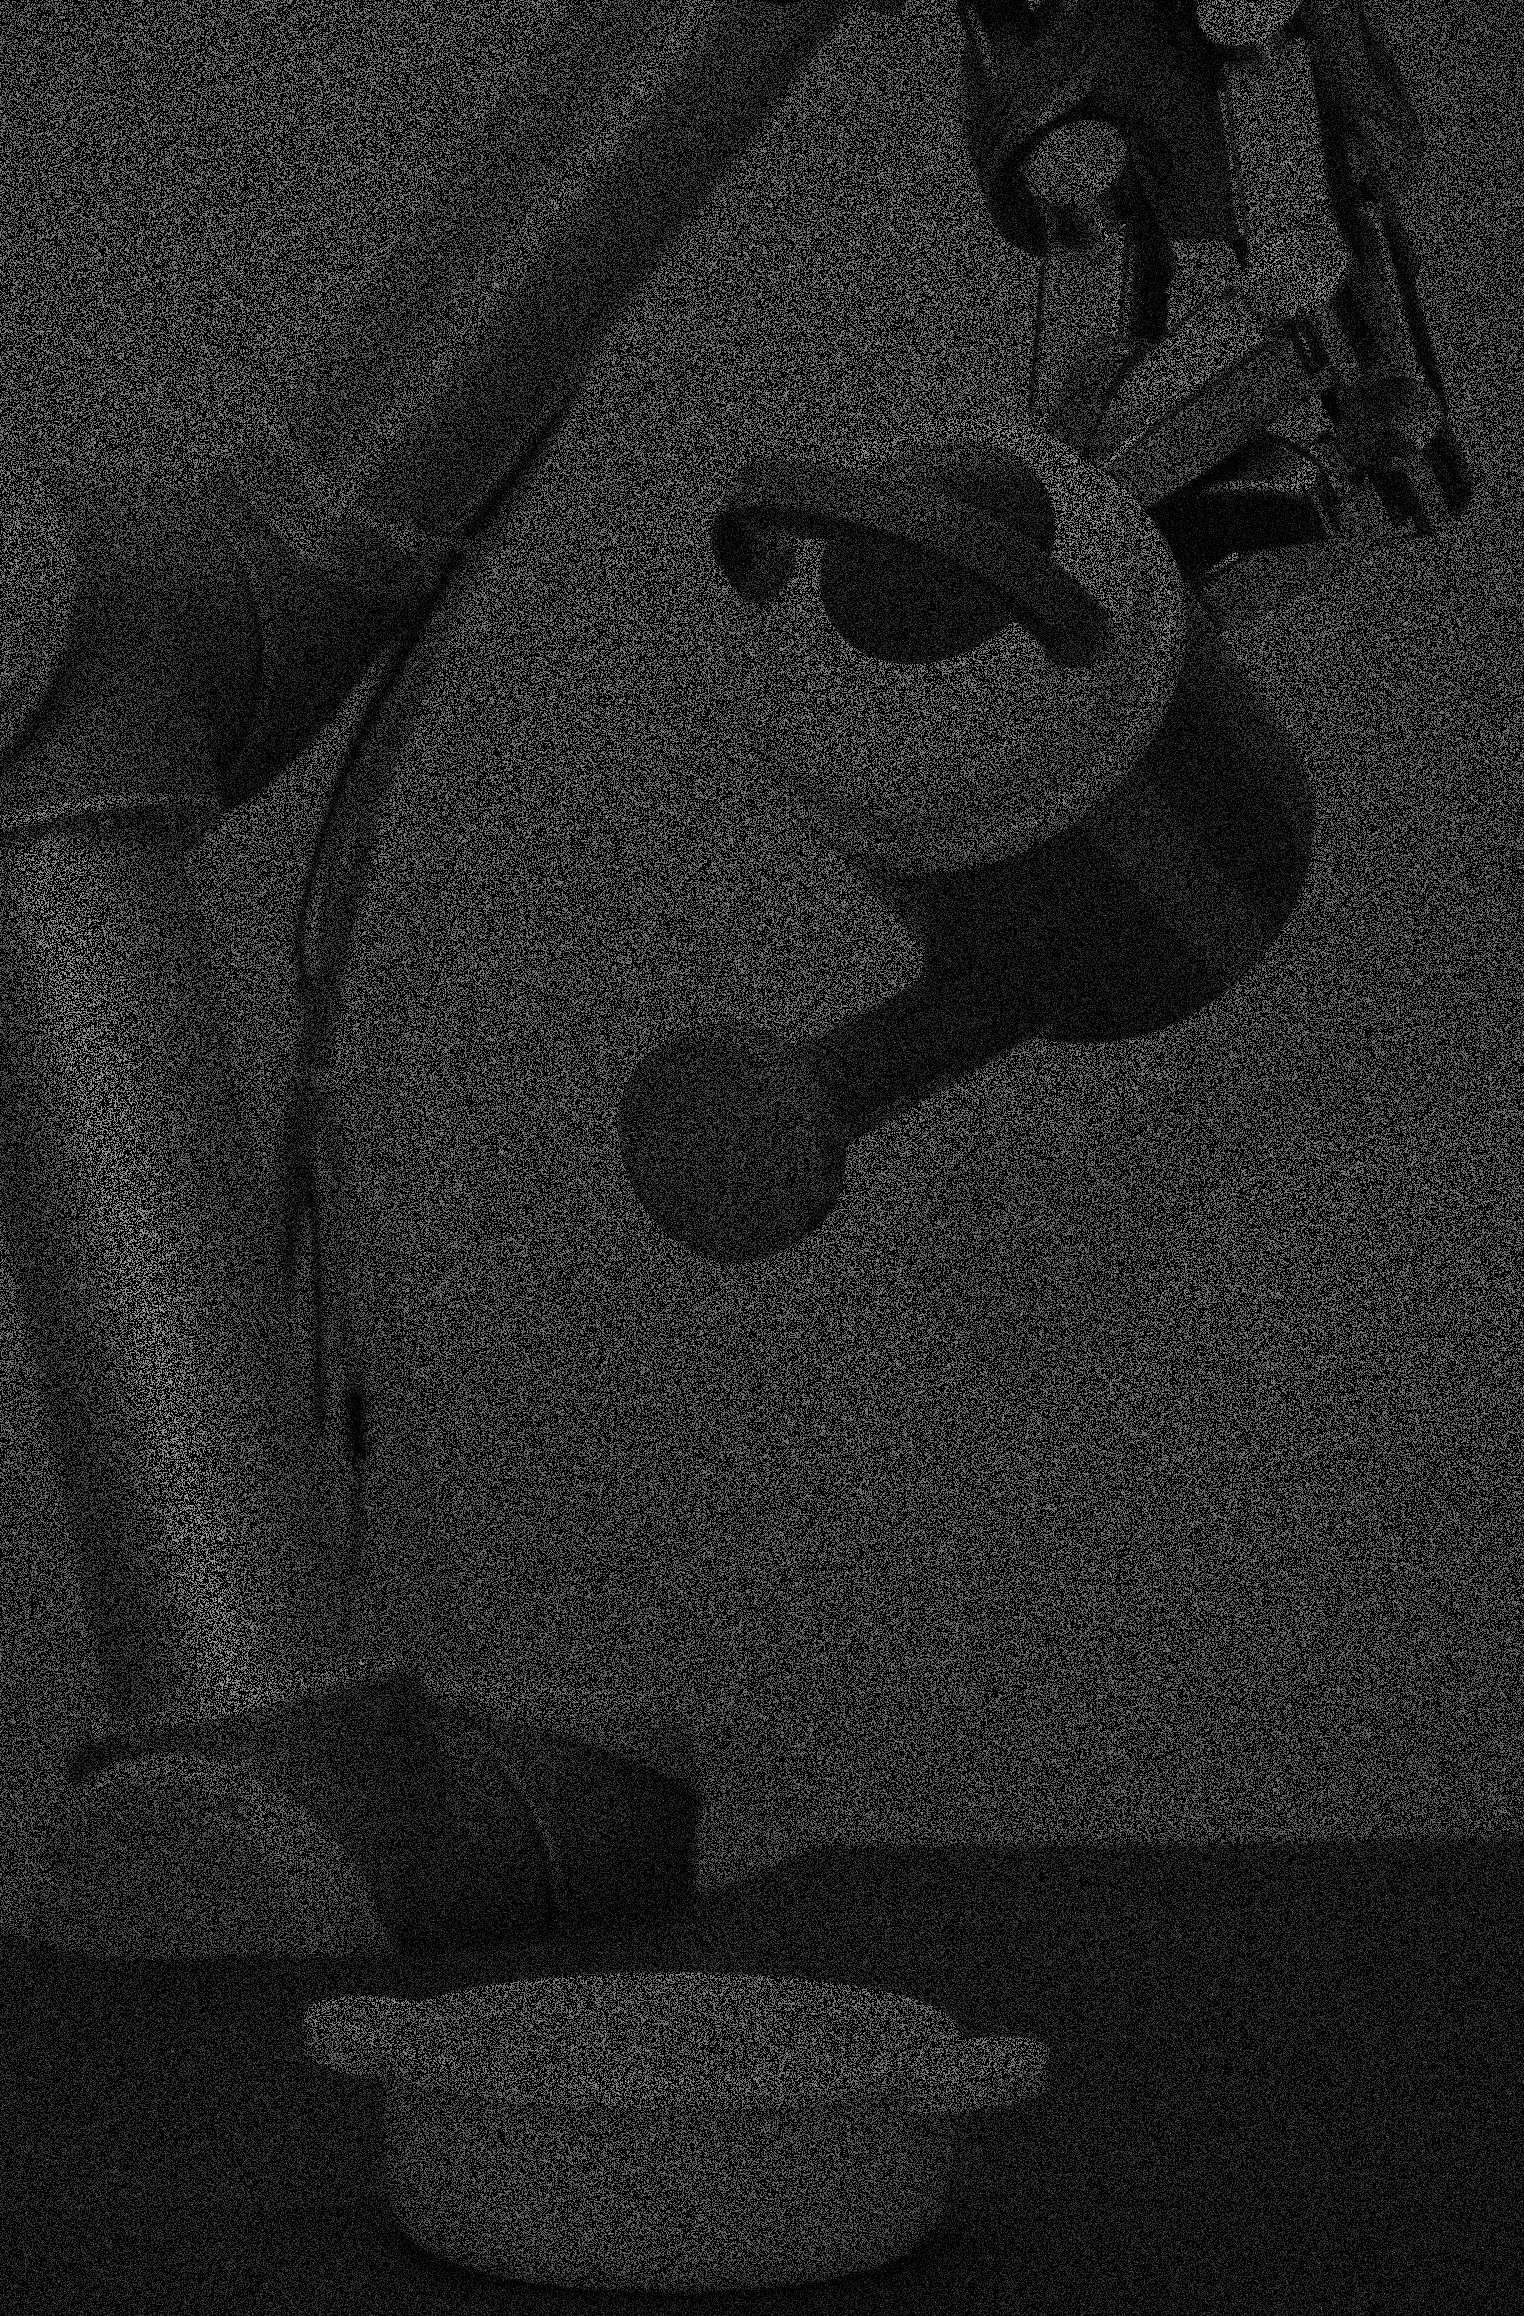
\includegraphics[width=\textwidth]{img1/Image1.png}
        \caption{Image1 with \\no restoration}
        \label{fig:img1_src}
    \end{subfigure}
    \begin{subfigure}[b]{0.446\textwidth}
        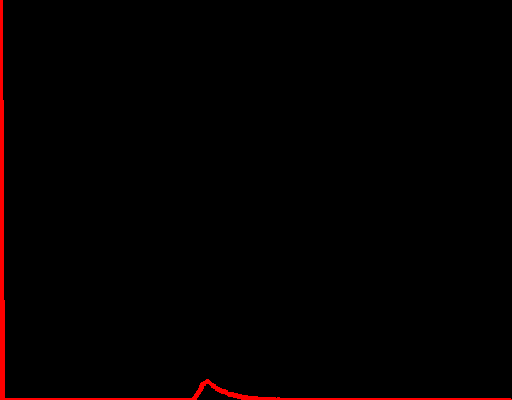
\includegraphics[width=\textwidth]{img1/src_hist1.png}
        \caption{Histogram of Image1}
        \label{fig:img1_hist}
    \end{subfigure}
    \caption{Analysis of image 1}\label{fig:img1}
\end{figure}

An effective way of removing salt and pepper noise it to use an median filter, which would take the median value  of fixed numbered  values and assign it to that pixel position, but as the amount of pepper noise is too large, will an median value mostly likely lead to a black pixel, thus not provide that much of an improvement as seen in Figure \ref{fig:img_median_full}.  

\begin{figure}[H]
    \centering
    \begin{subfigure}[b]{0.27\textwidth}
        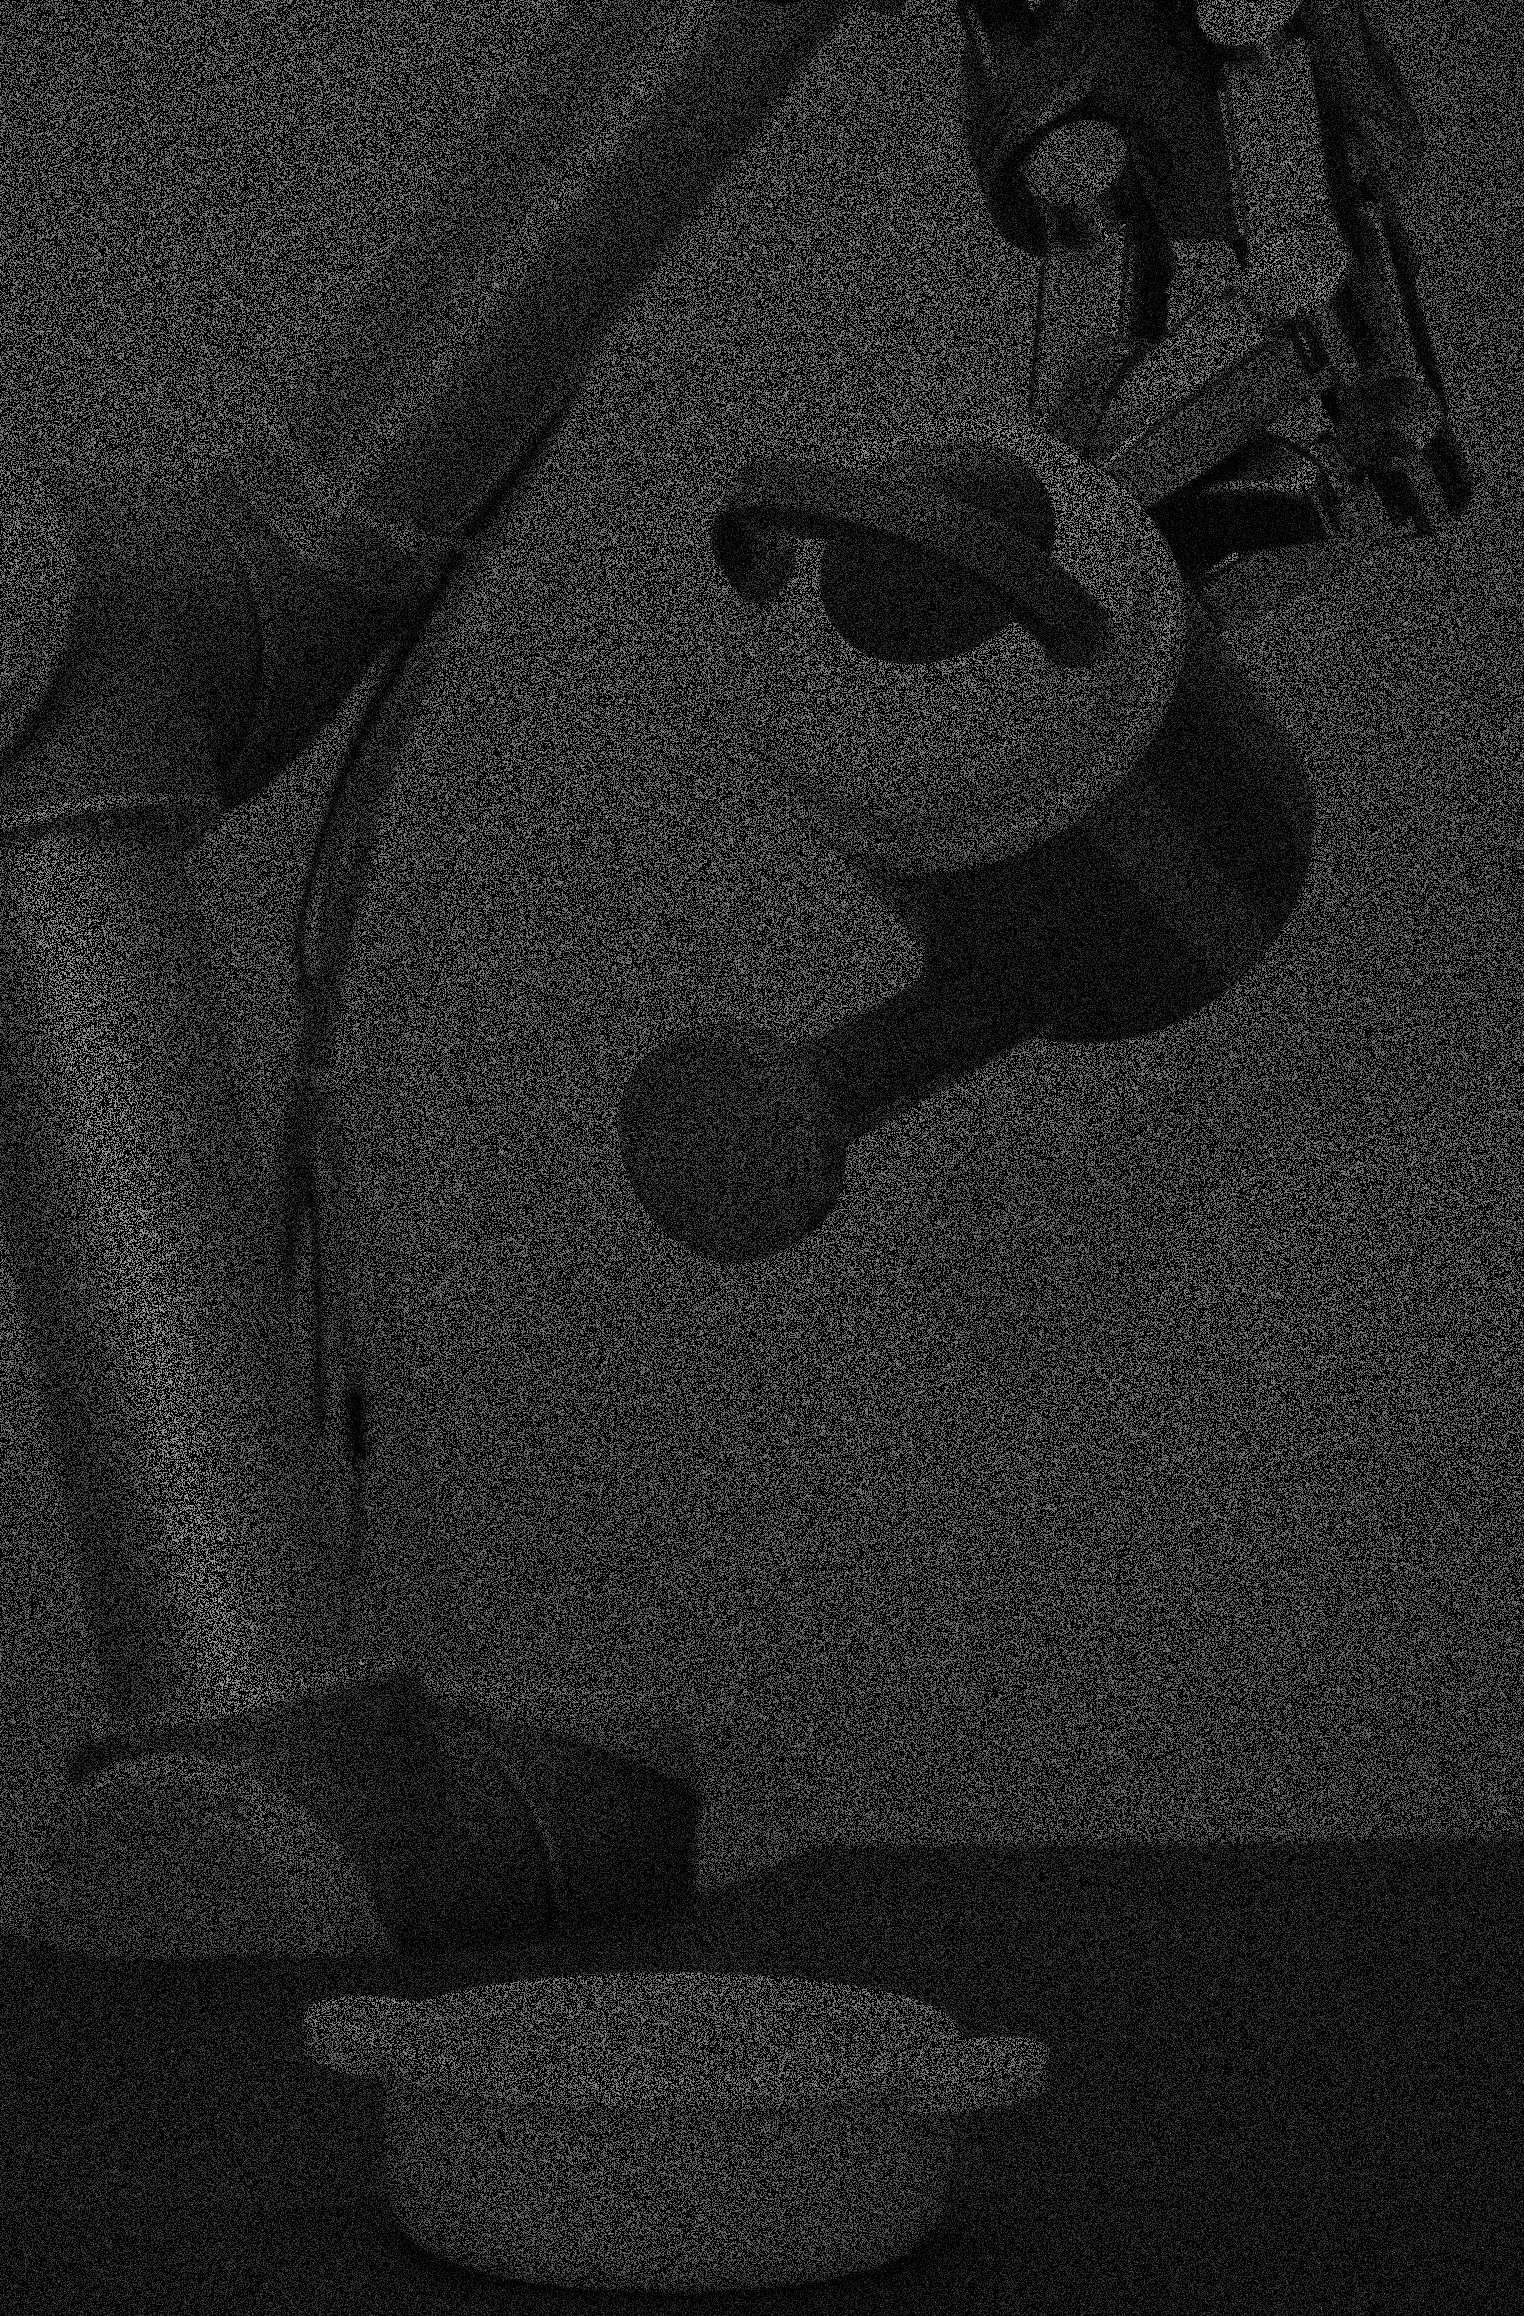
\includegraphics[width=\textwidth]{img1/Image1.png}
        \caption{Image1 with \\no restoration}
    \end{subfigure}
    \begin{subfigure}[b]{0.27\textwidth}
        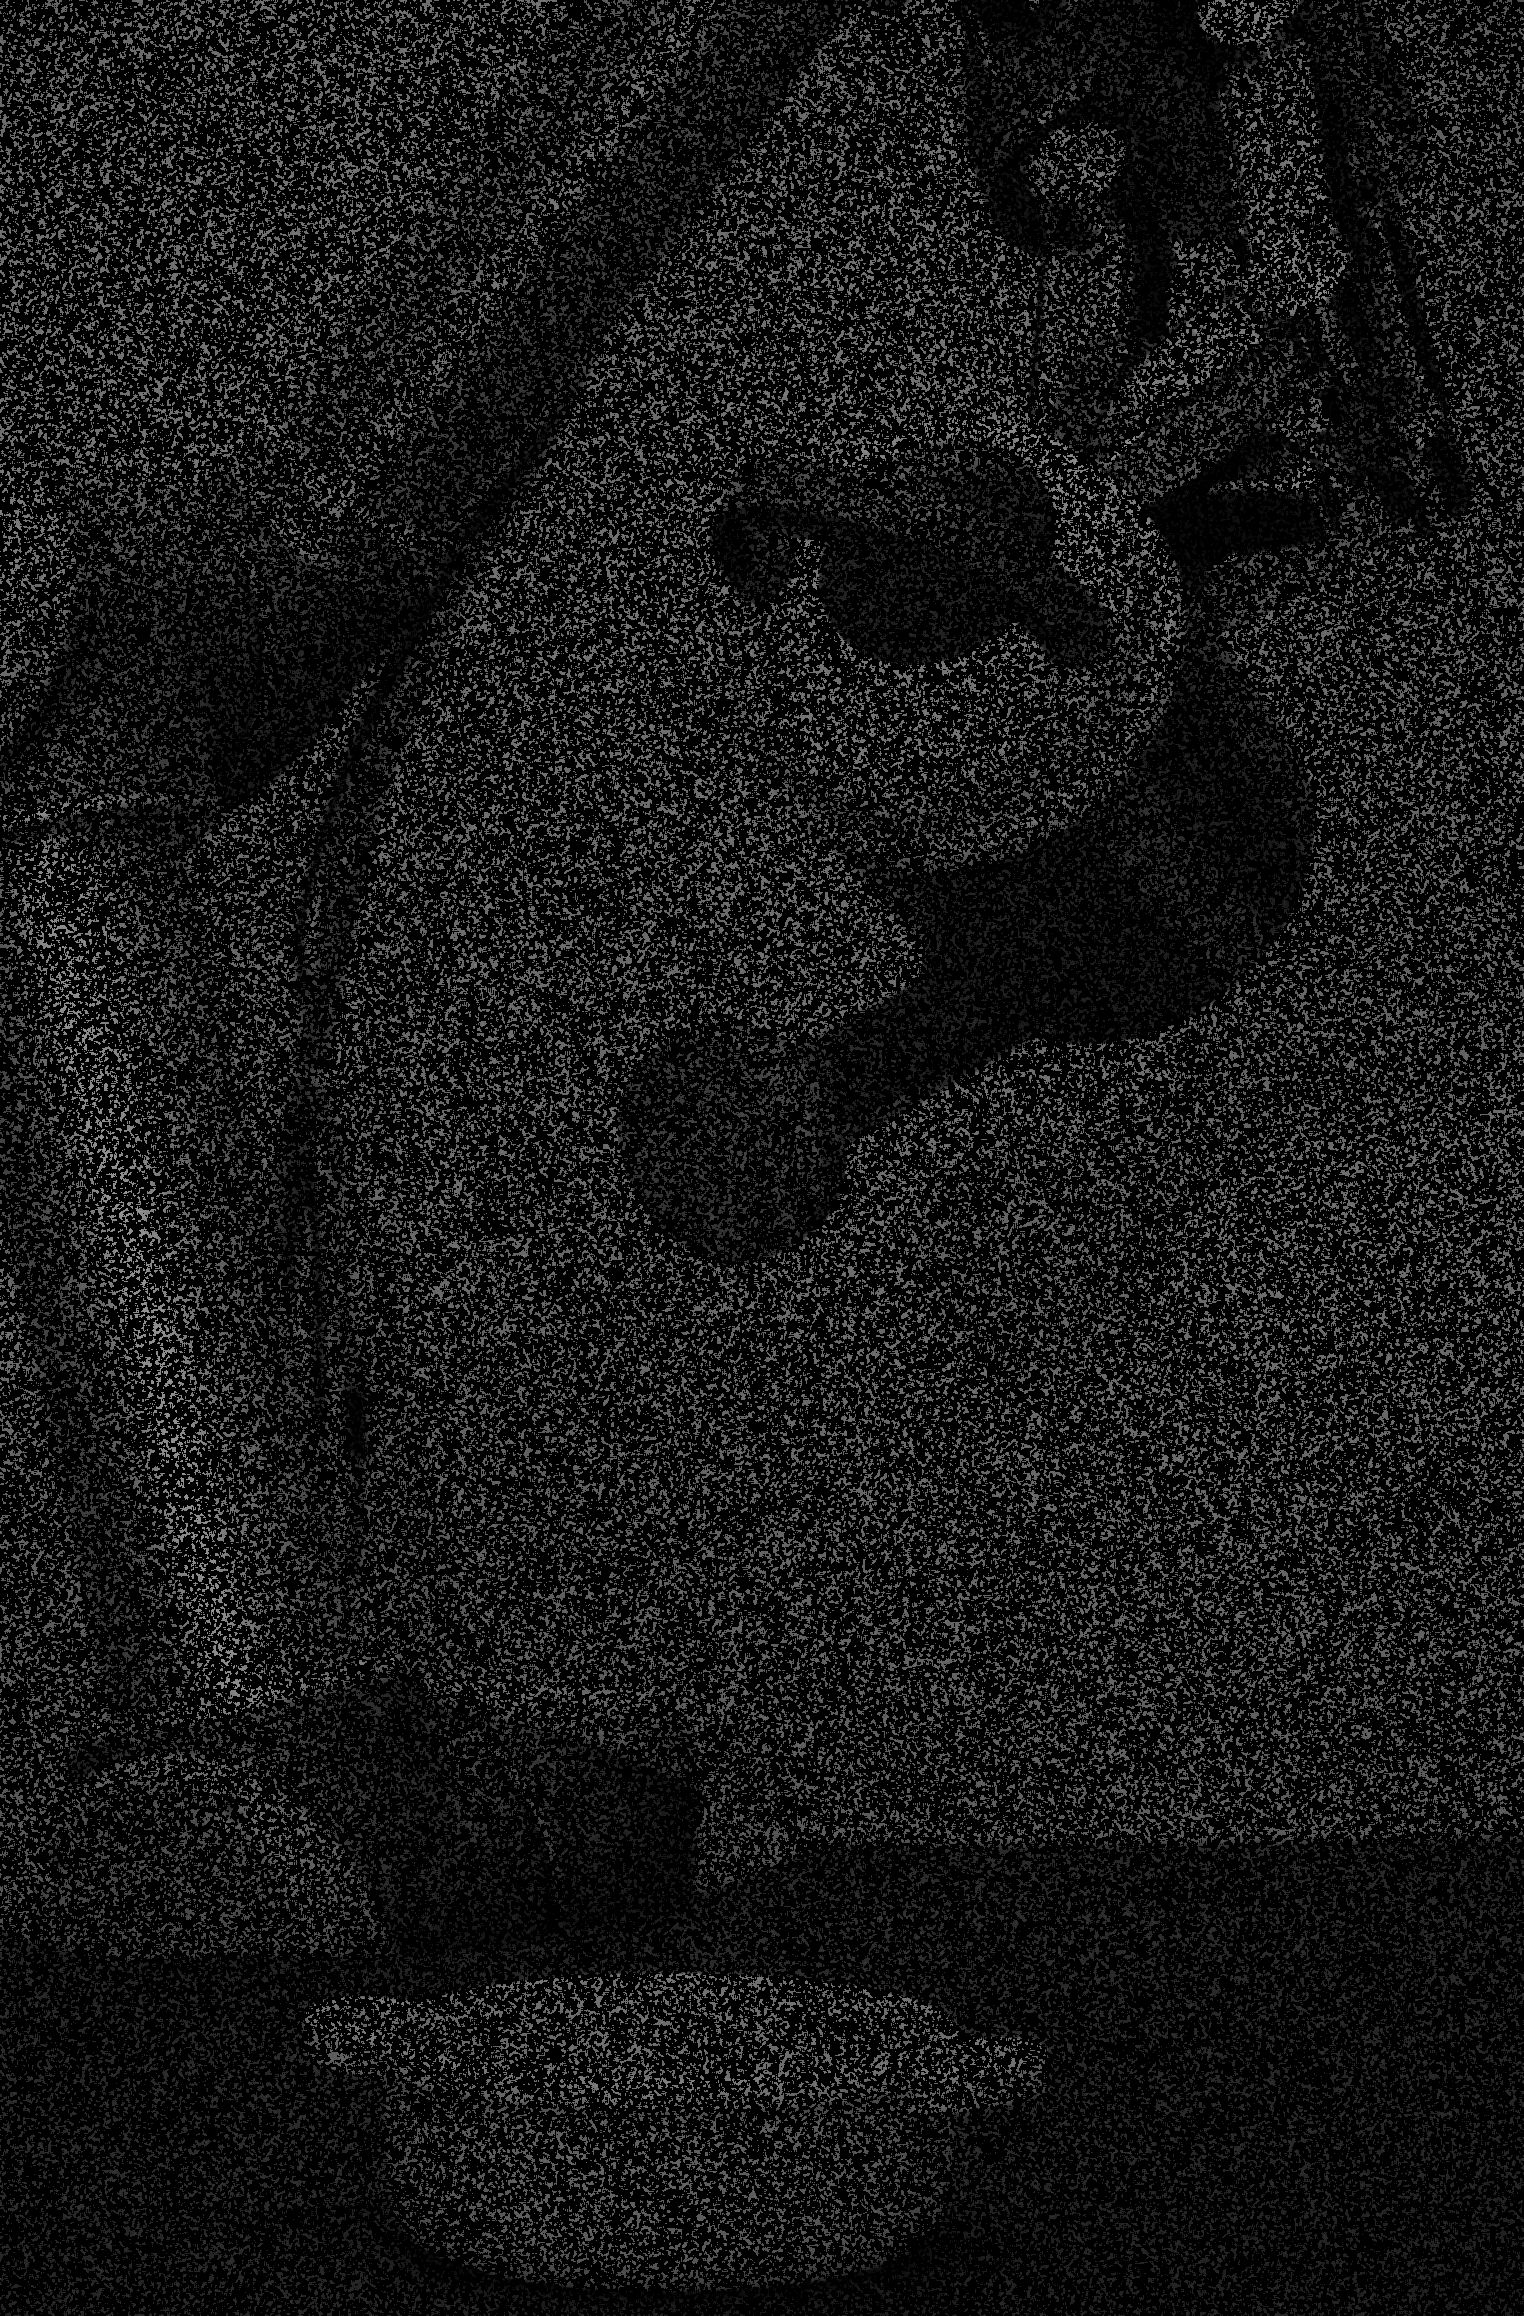
\includegraphics[width=\textwidth]{img1/img_1_medianBlur_3.png}
        \caption{Image1 filtered with median filter kernelsize 3}
        \label{fig:img1_median3}
    \end{subfigure}
       \begin{subfigure}[b]{0.27\textwidth}
        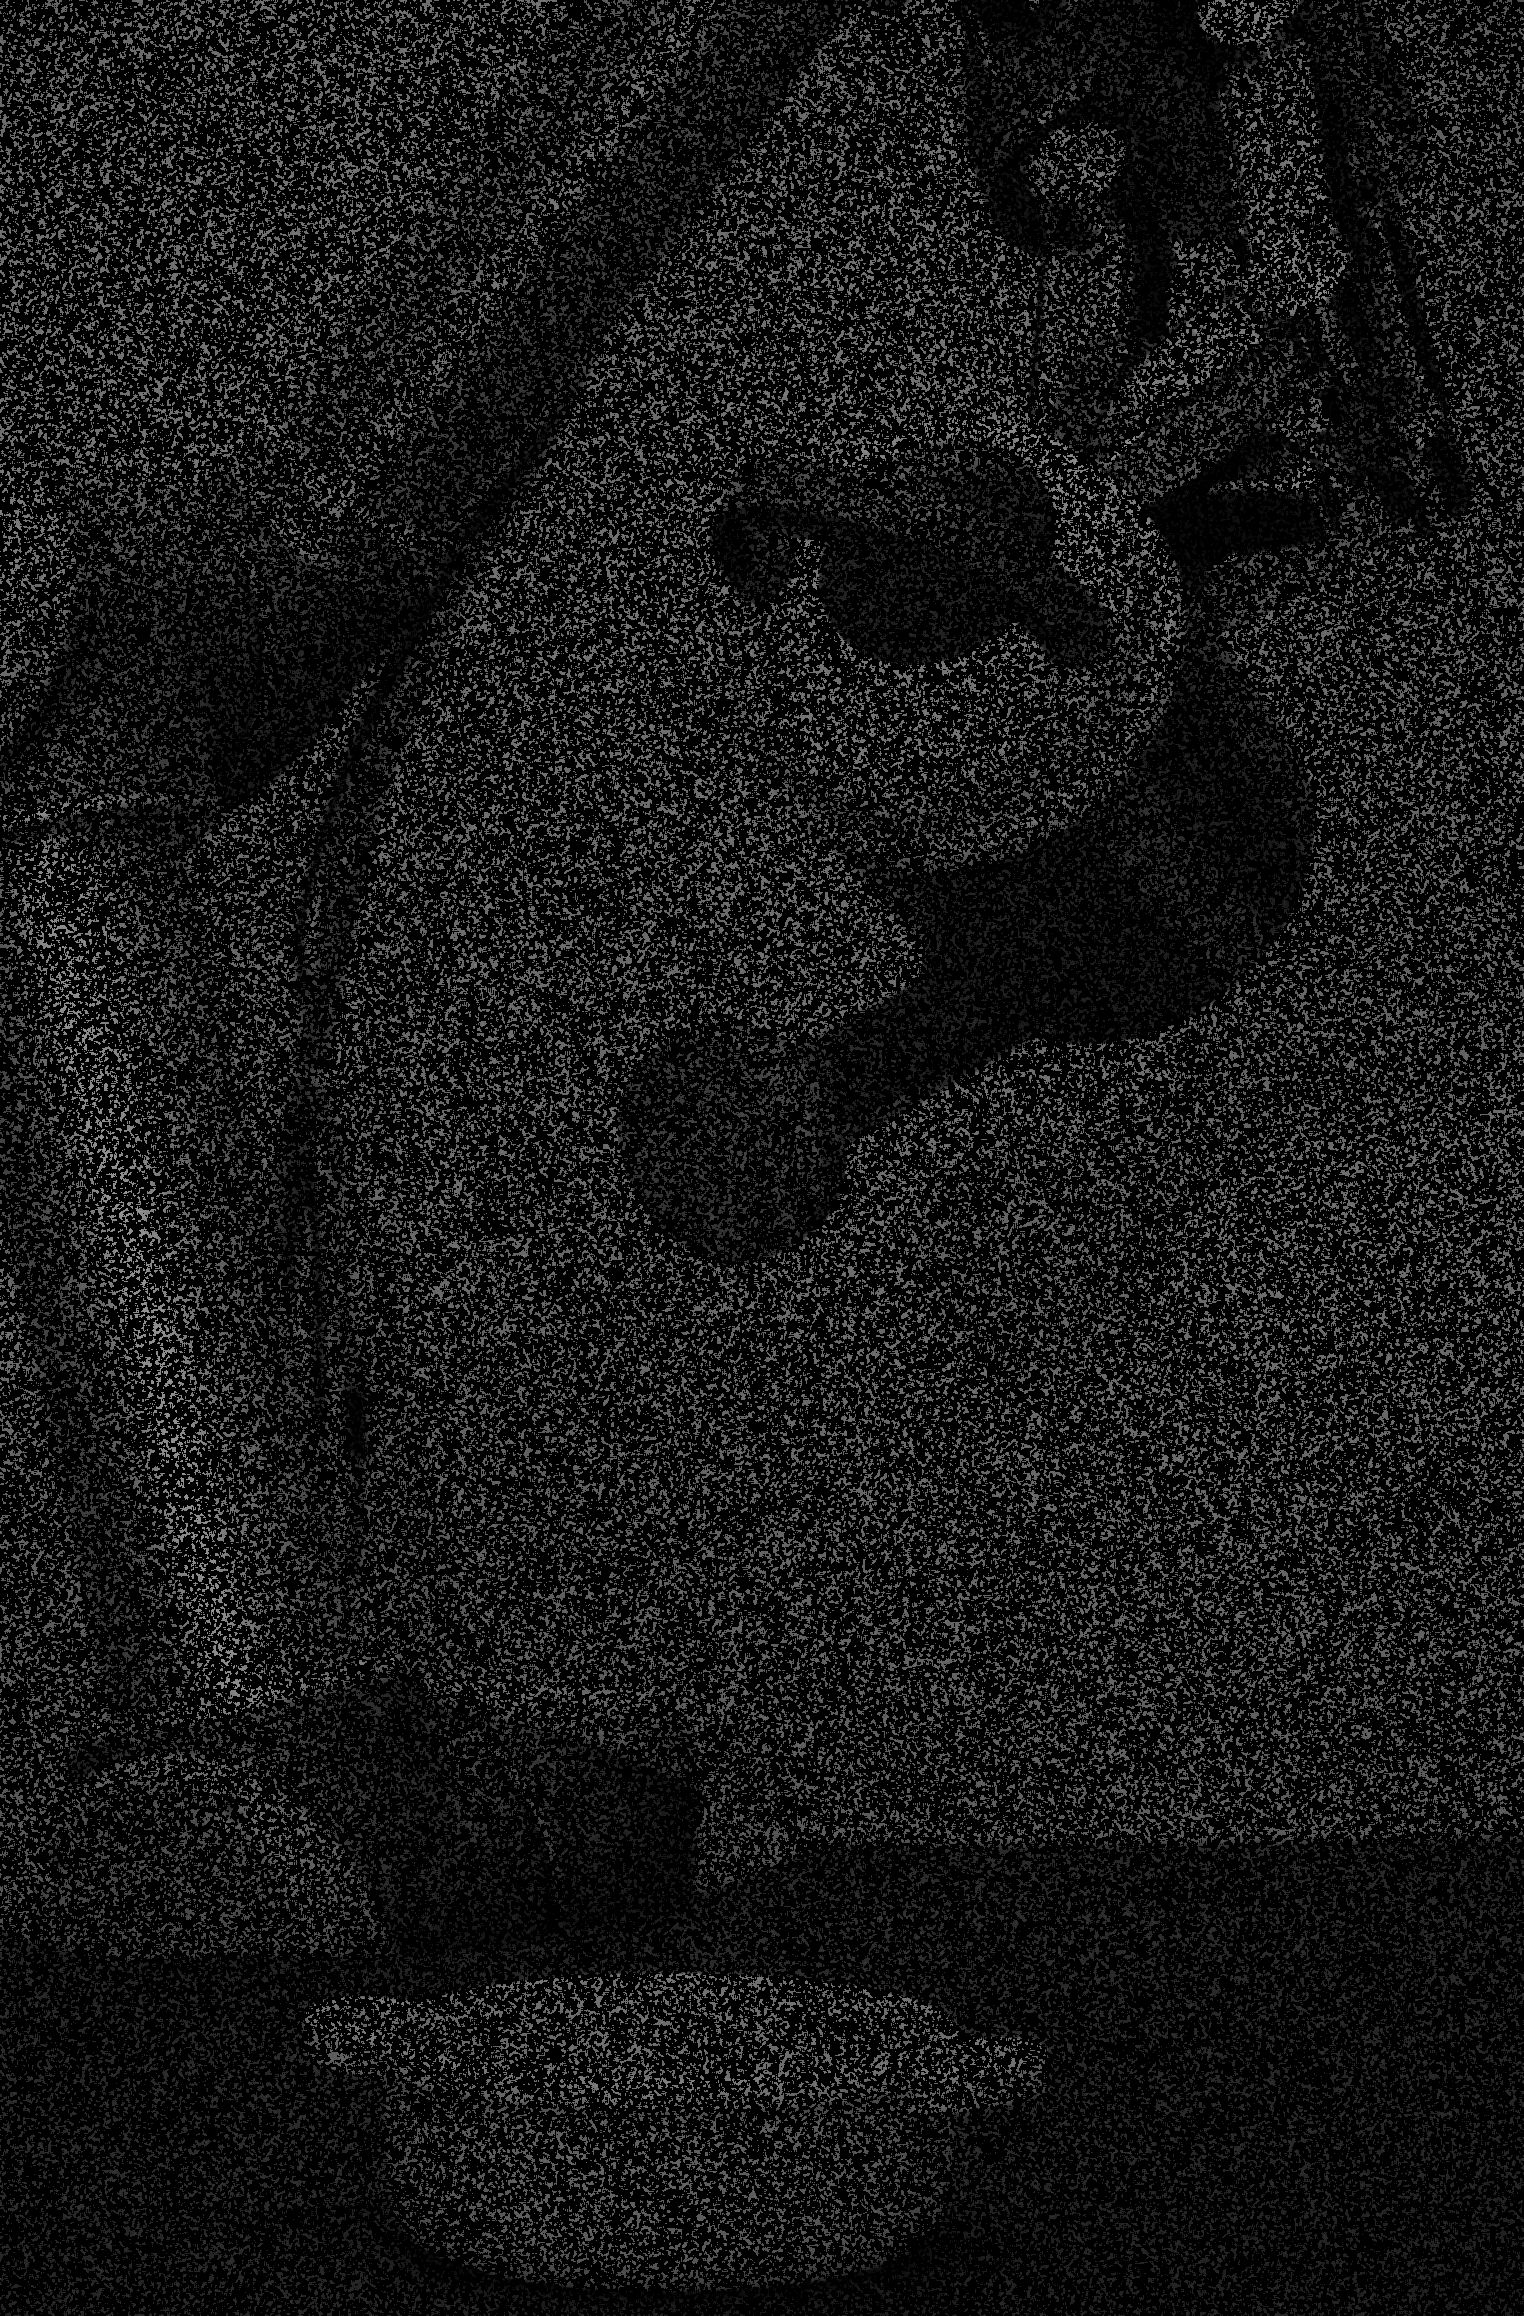
\includegraphics[width=\textwidth]{img1/img_1_medianBlur_9.png}
        \caption{Image1 filtered with median filter kernelsize 9}
        \label{fig:img1_median9}
    \end{subfigure}
    \caption{Median filter applied to image1}\label{fig:img_median_full}
\end{figure}

As the Median filter did not show  any form of improvement, an other method had to be used instead.  An Contraharmonic mean filter implemented and tried.  

An contraharmonic mean filter restores an images using this expression
\begin{equation}
\hat{f}(u,v) = \frac{\sum\limits_{(s,t) \in S_{xy}}g(s,t)^{Q+1}}{\sum\limits_{(s,t) \in S_{xy}}g(s,t)^{Q}}
\cite{Image processing Bogen p. 345}
\label{eq:Contra}
\end{equation}
\todo{citation has to be added to the book p. 345}

In Equation \ref{eq:Contra}, is $S_{xy}$ a rectangular  window with a center pixel. $g$ is the corrupted images, and $\hat{f}$ is the restored image. $Q$ defines the order of the filter.  \\
The filter is suited for removing salt and pepper noises. The filter reduce the effect of pepper noise for positive Q values, and Salt noise for negative Q values. it can also be reduced to an arithmetic filter by setting $Q = 0$ or harmonic filter by setting $Q = -1$. The filter was implemented due to its multiple applicability, and applied on Figure \ref{fig:img1_src} with different positive value which the result can bee seen on Figure \ref{fig:img1_contra}, to test how well it well it could restore the image to its original condition.  

\begin{figure}[H]
    \centering
    \begin{subfigure}[b]{0.3\textwidth}
        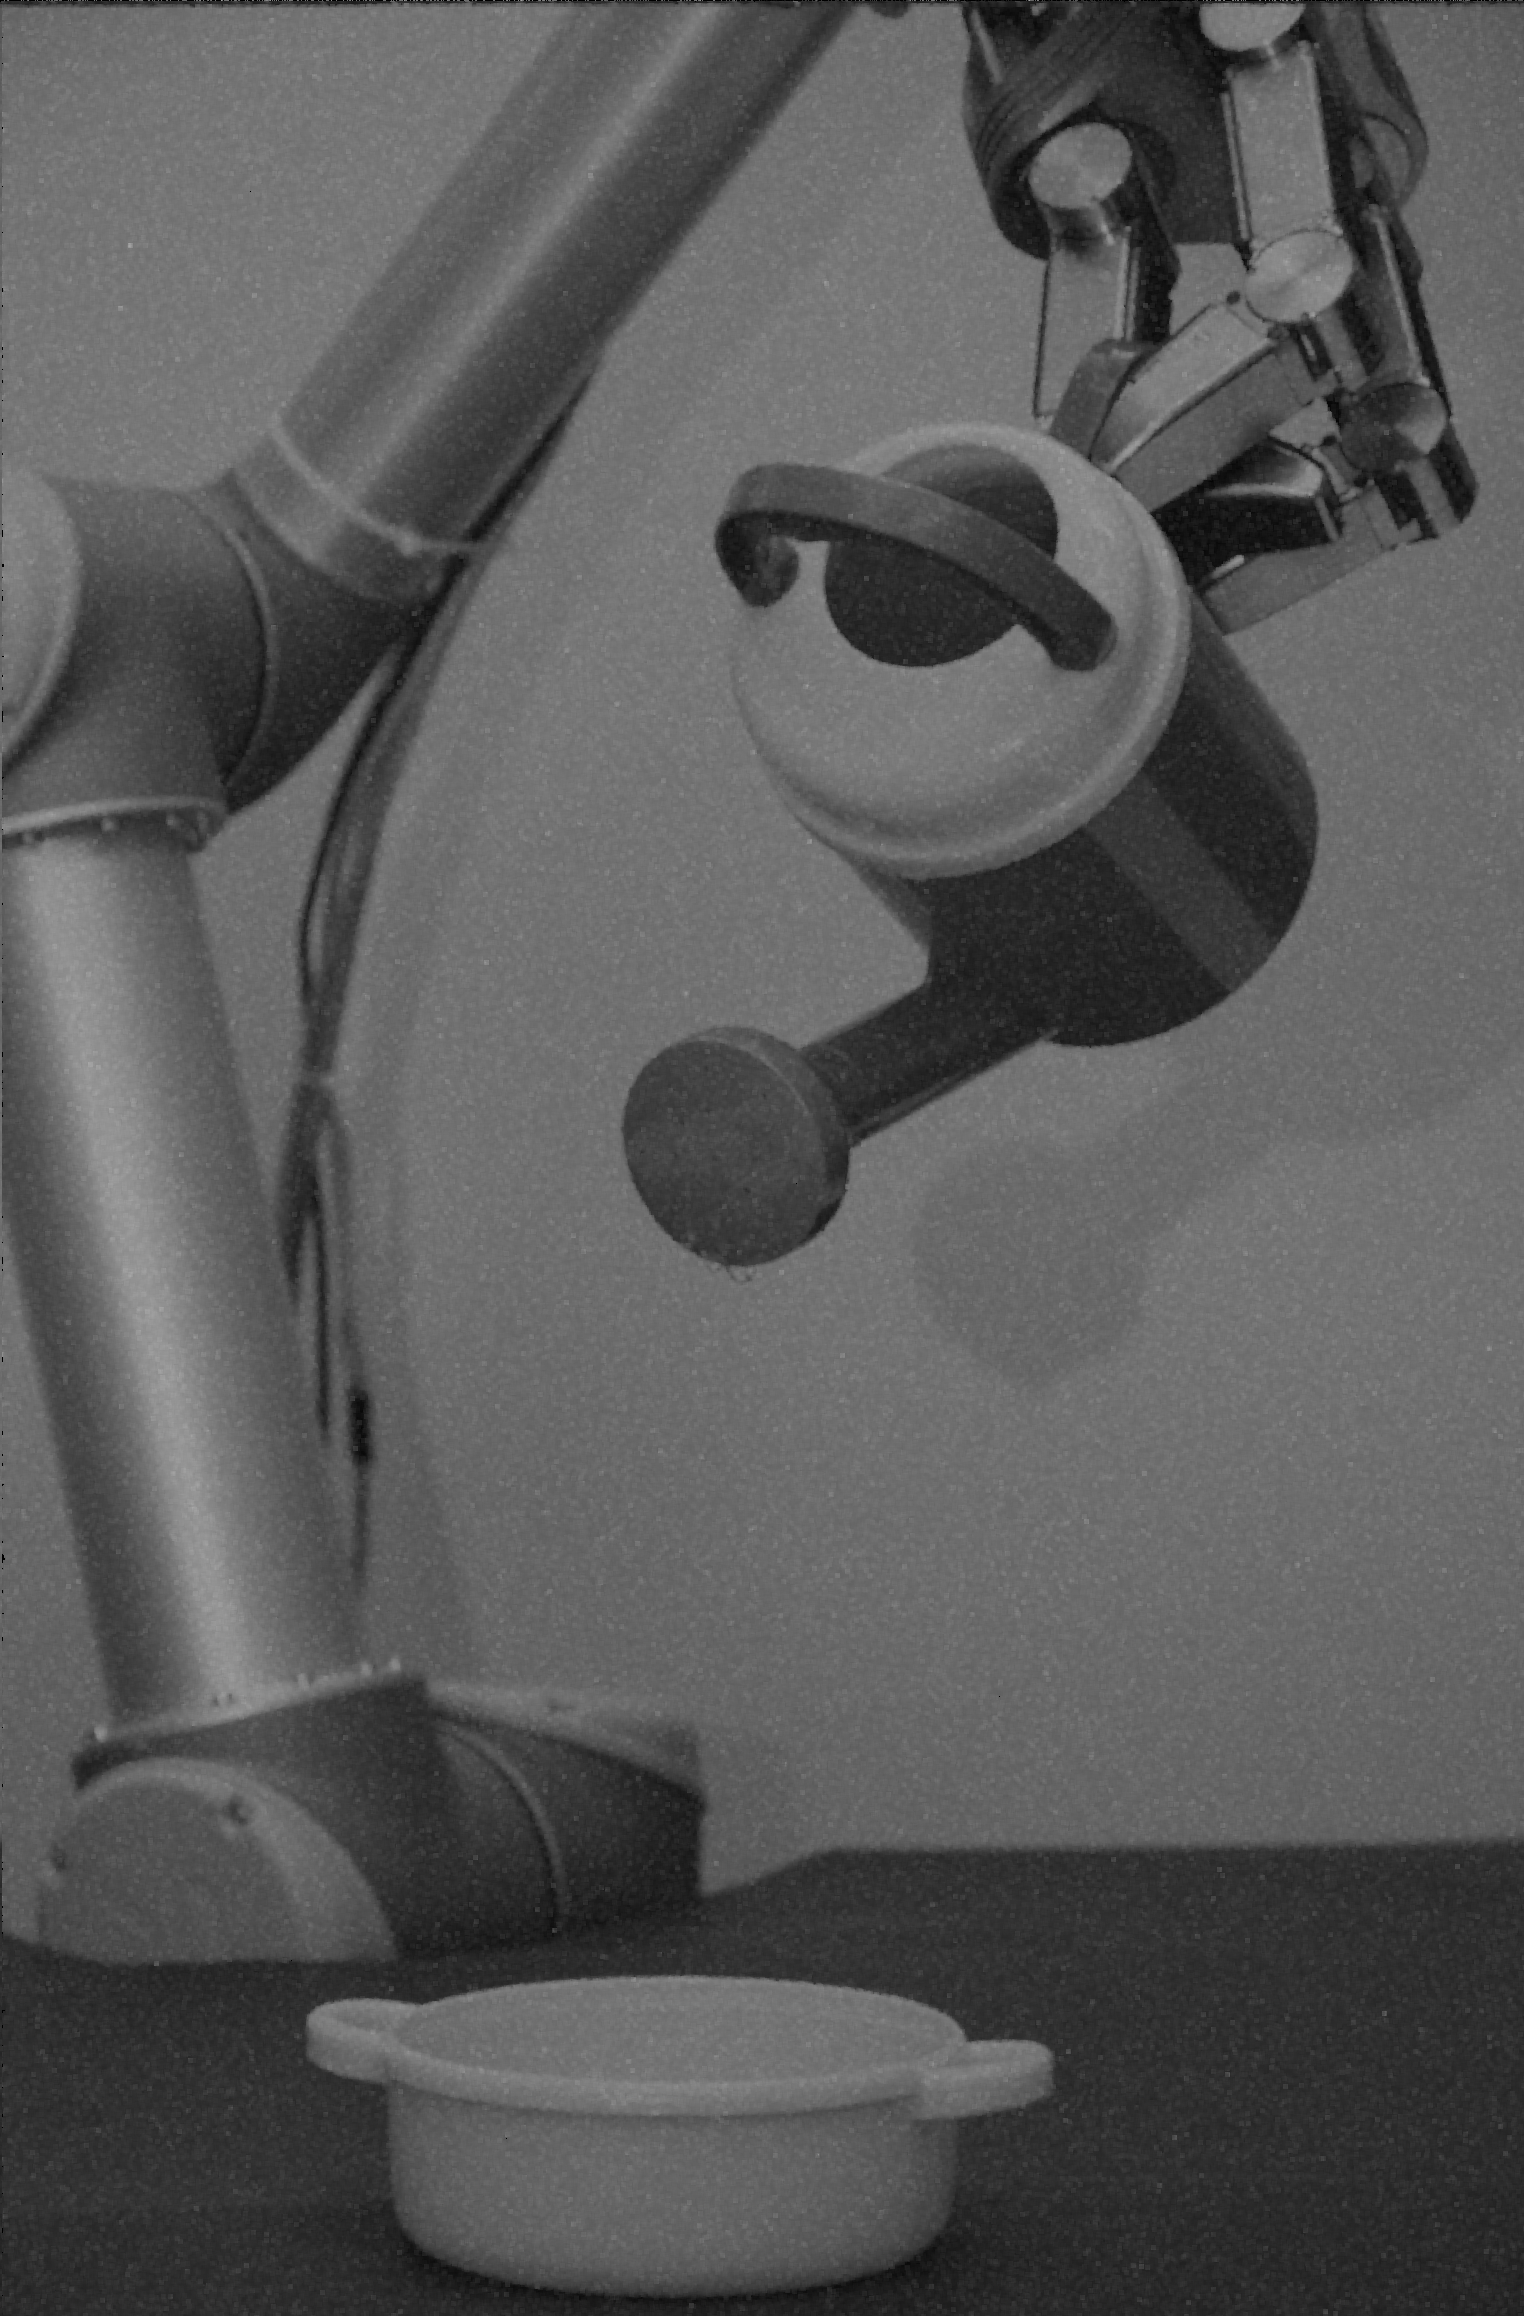
\includegraphics[width=\textwidth]{img1/img_1_gaus_5_1.png}
        \caption{Kernelsize: 5 order: 1}
          \label{fig:img1_contra5_1}
    \end{subfigure}
    \begin{subfigure}[b]{0.3\textwidth}
        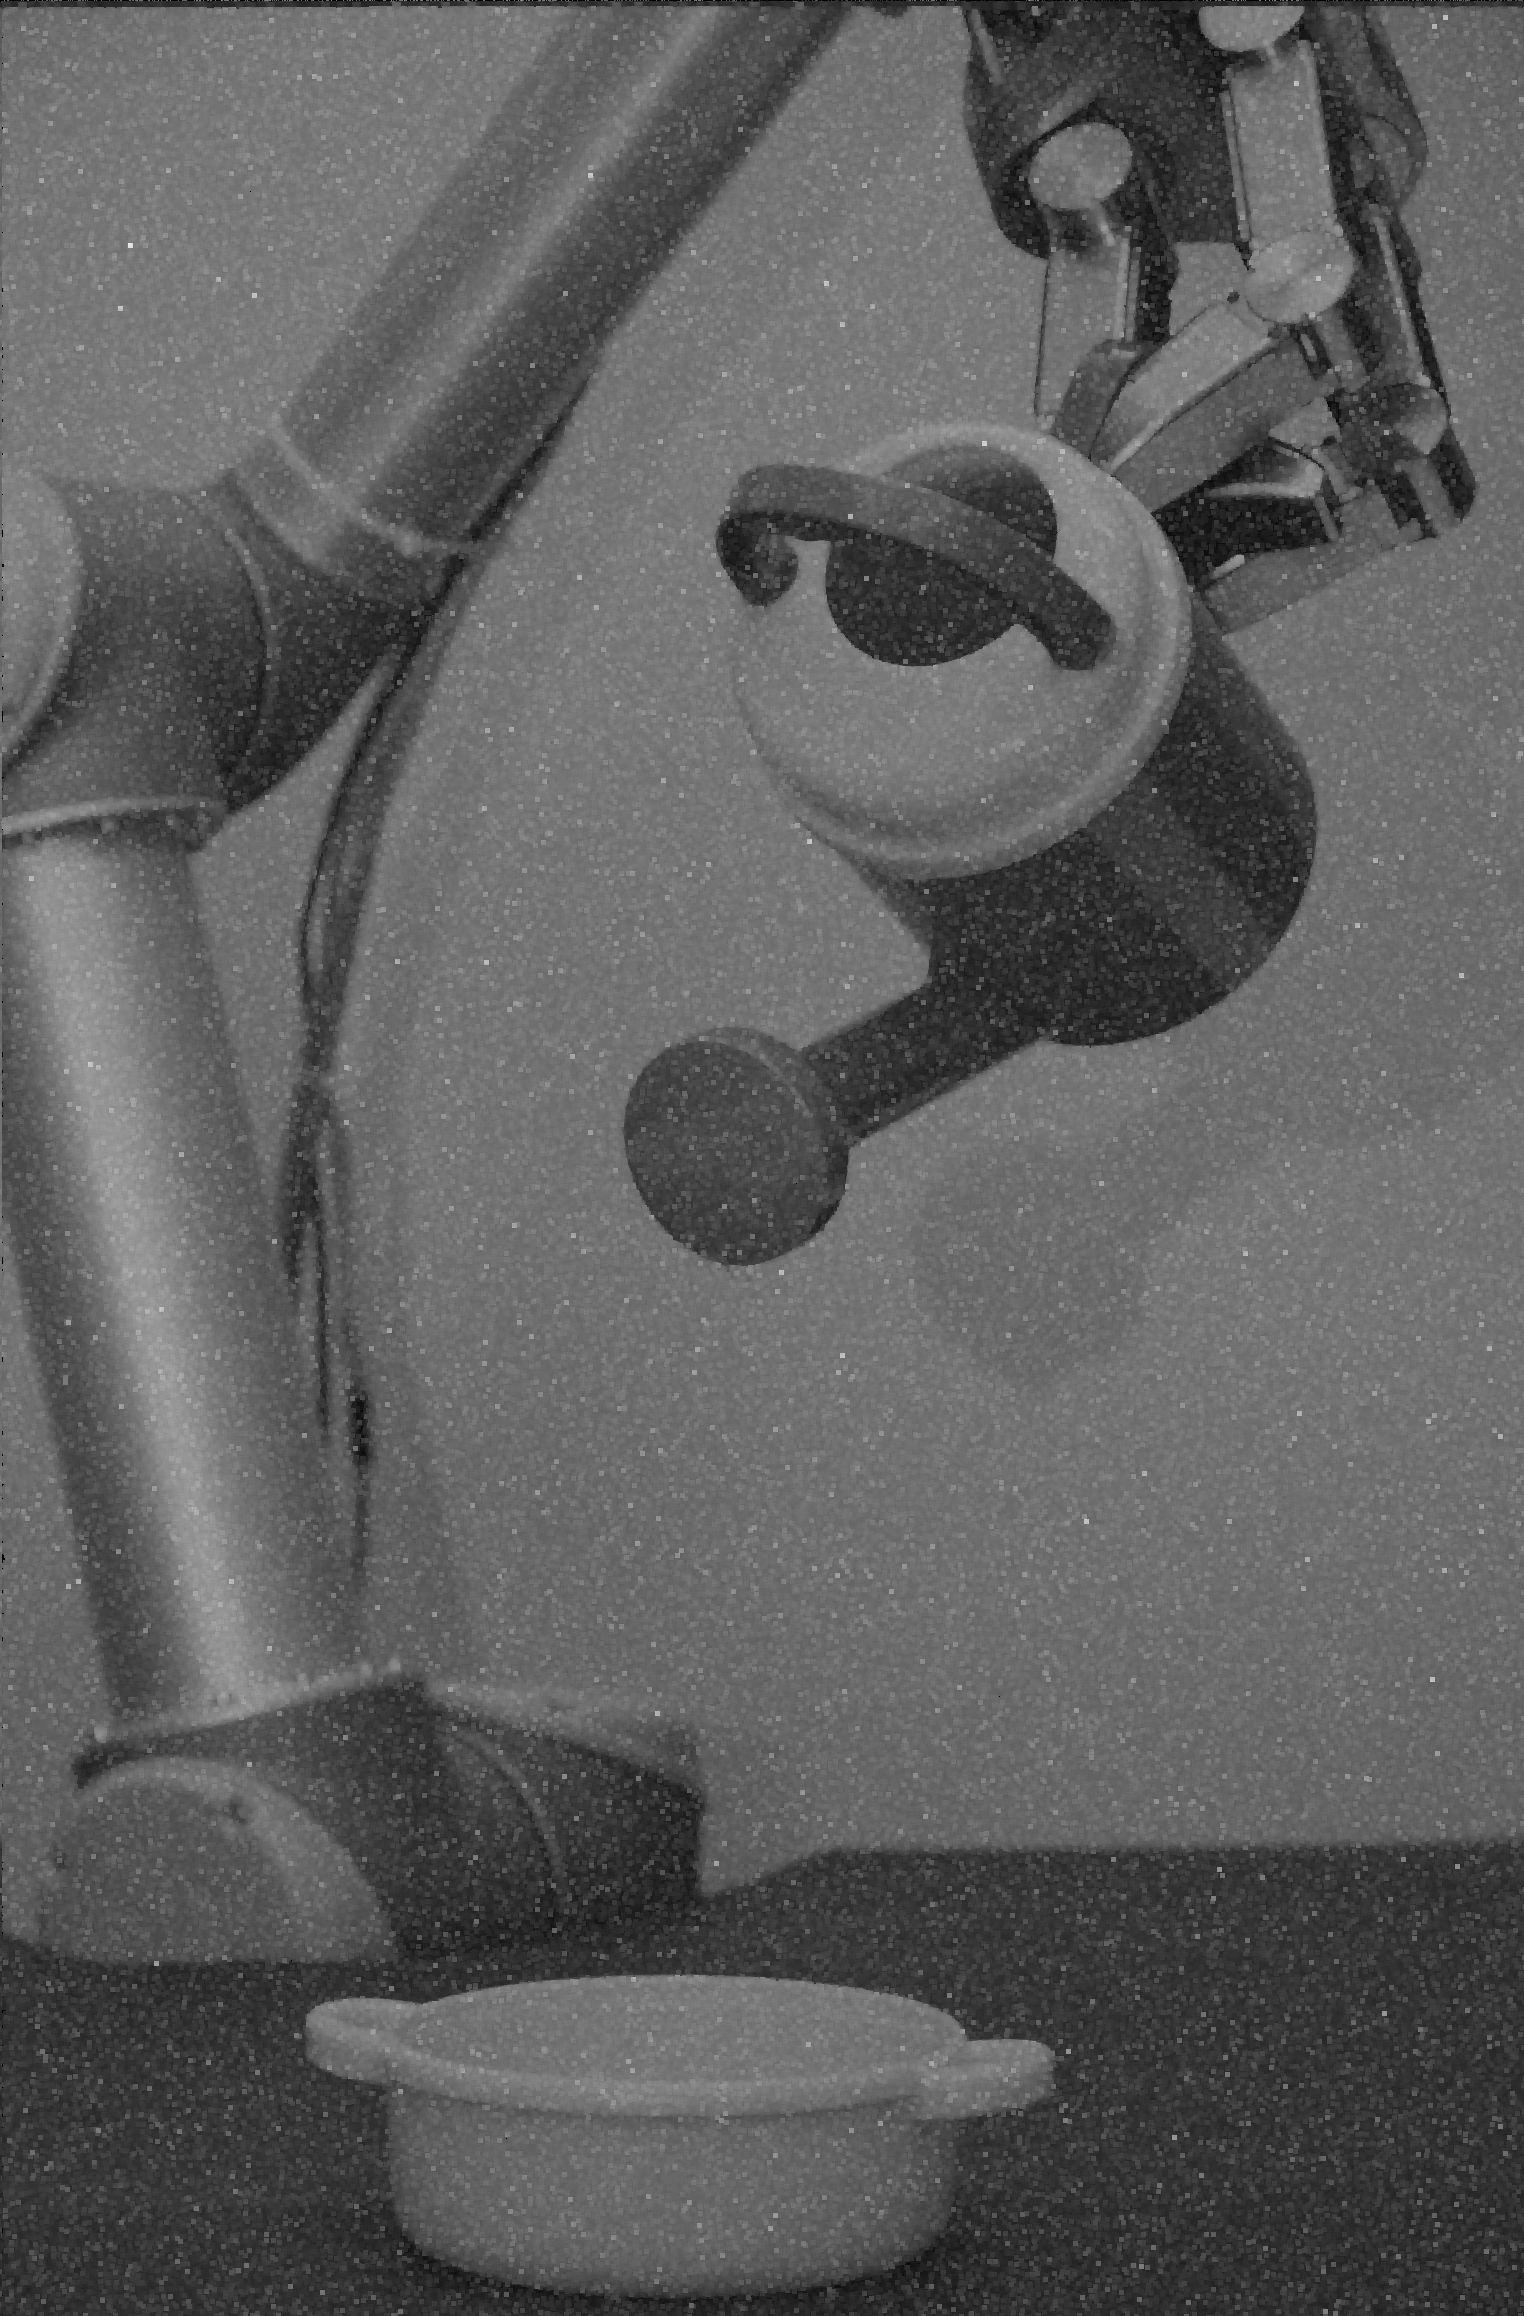
\includegraphics[width=\textwidth]{img1/img_1_gaus_5_5.png}
        \caption{Kernelsize: 5 order: 5}
          \label{fig:img1_contra5_5}
    \end{subfigure}
       \begin{subfigure}[b]{0.3\textwidth}
        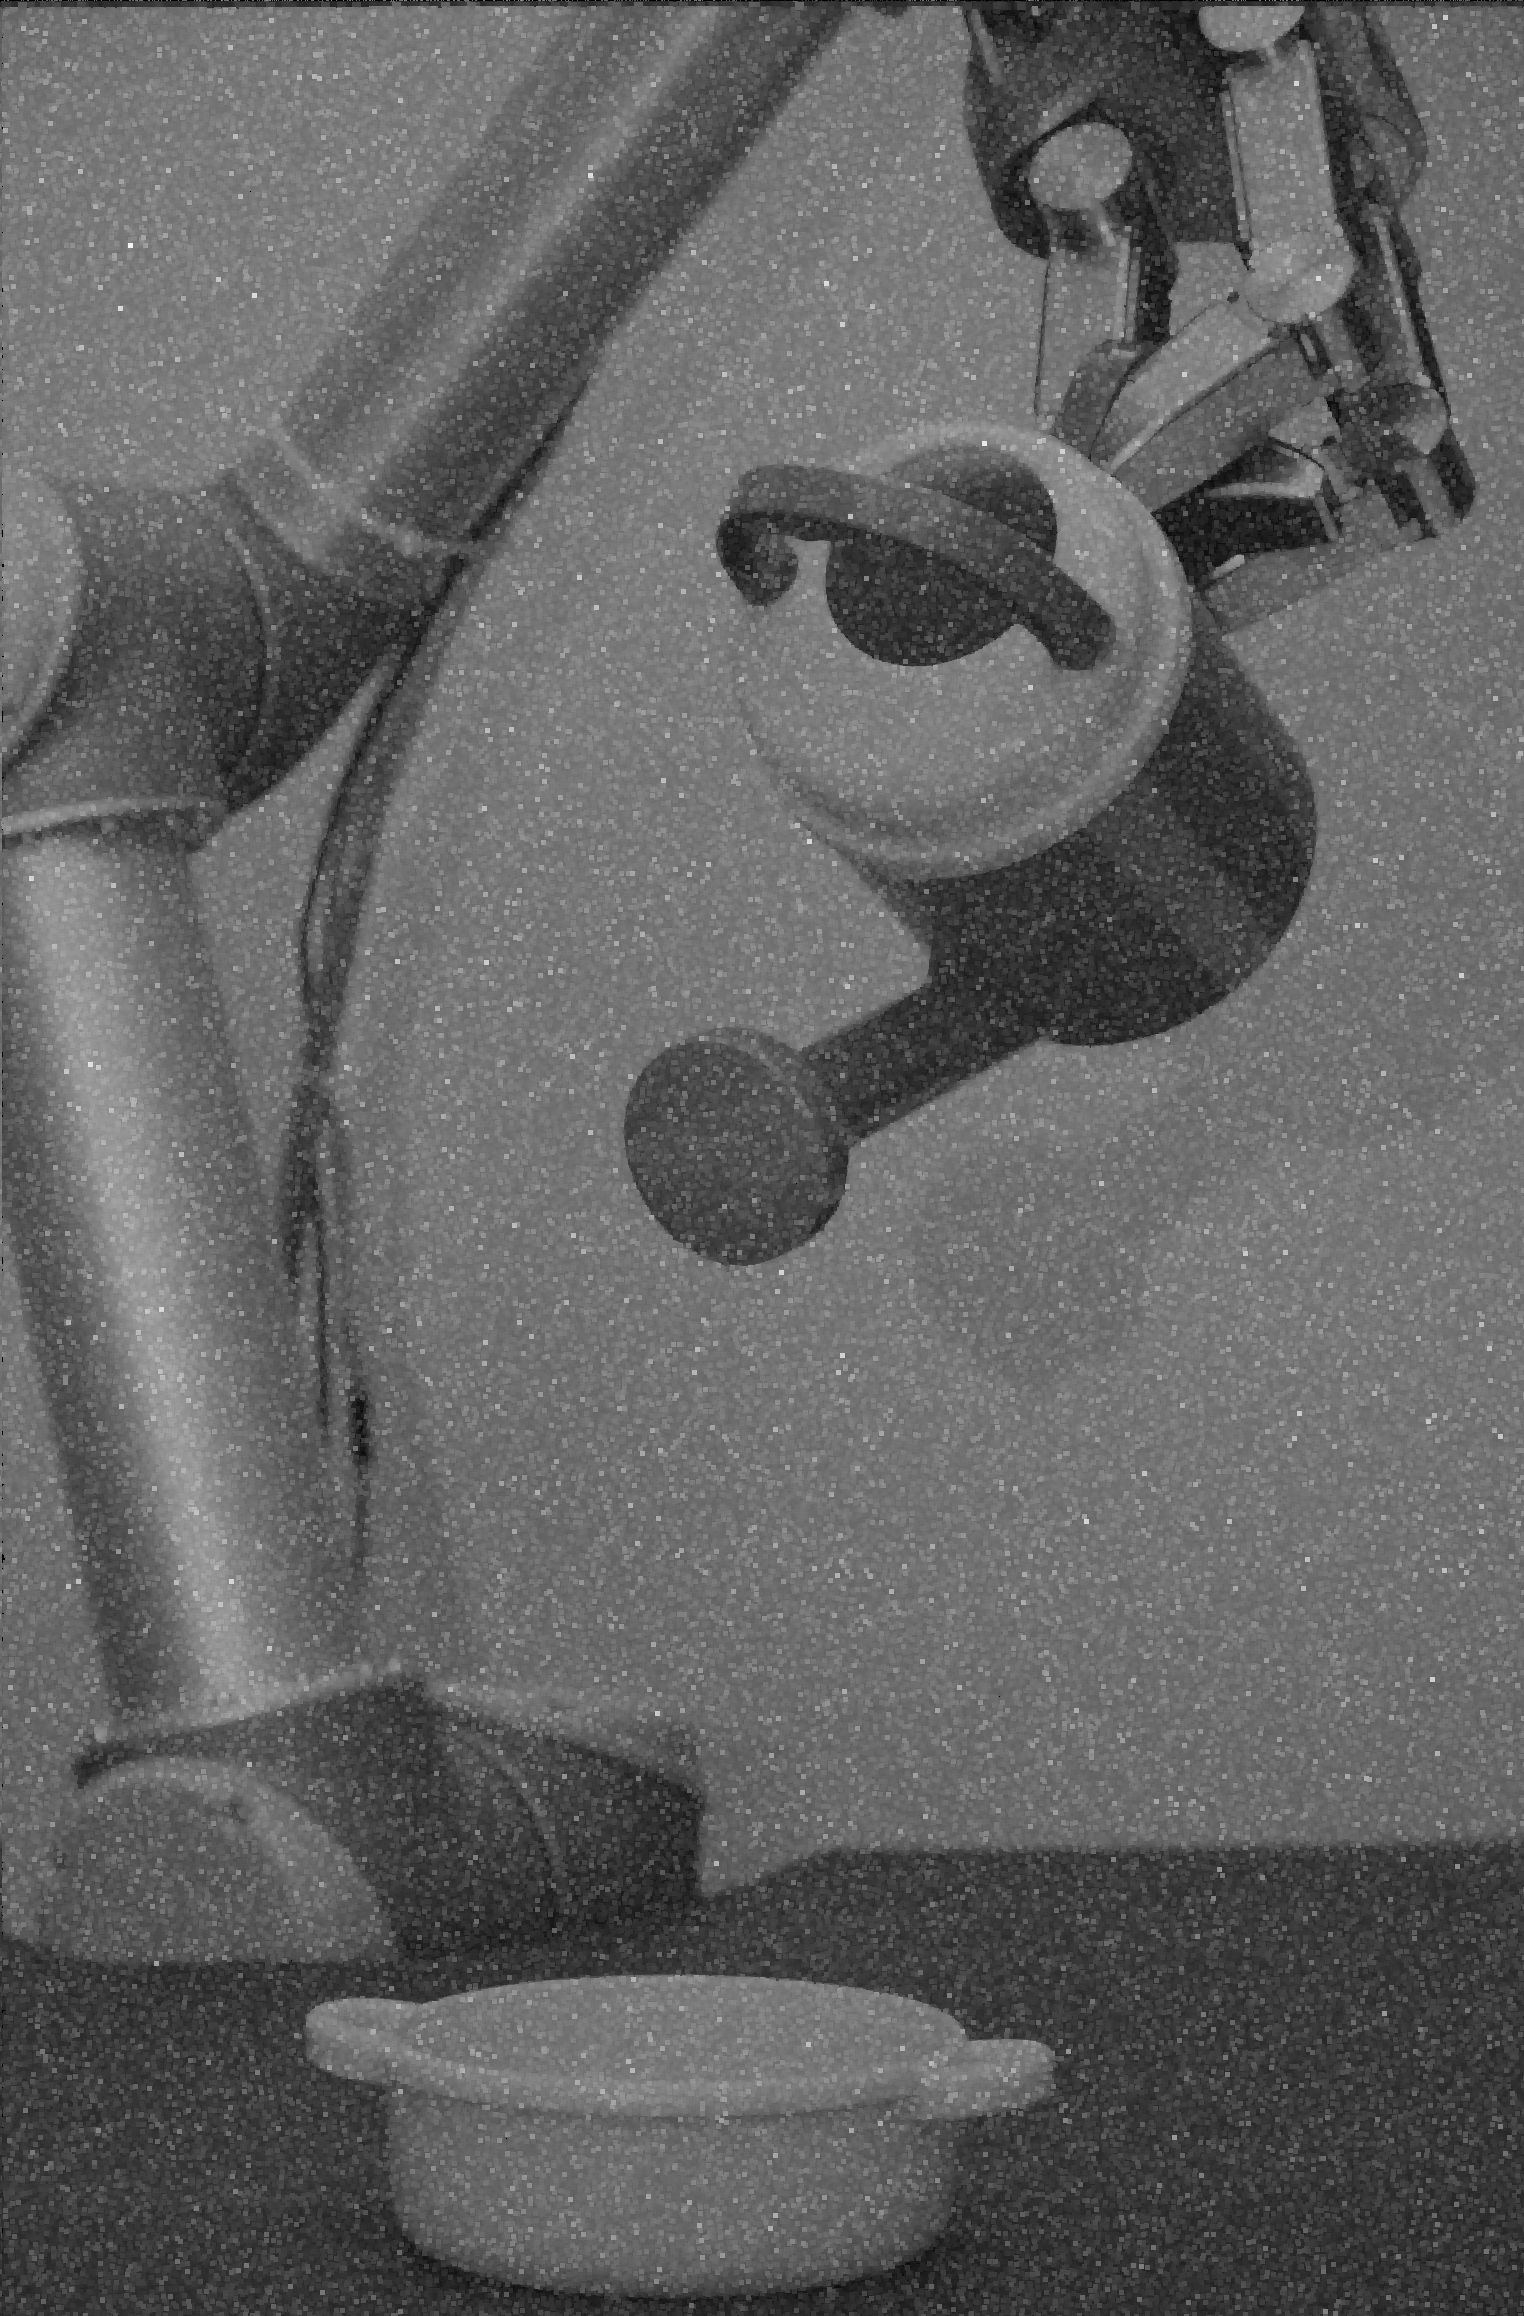
\includegraphics[width=\textwidth]{img1/img_1_gaus_5_9.png}
        \caption{Kernelsize: 5 order: 9}
          \label{fig:img1_contra5_9}
    \end{subfigure}
    
    
    
    
       \begin{subfigure}[b]{0.3\textwidth}
        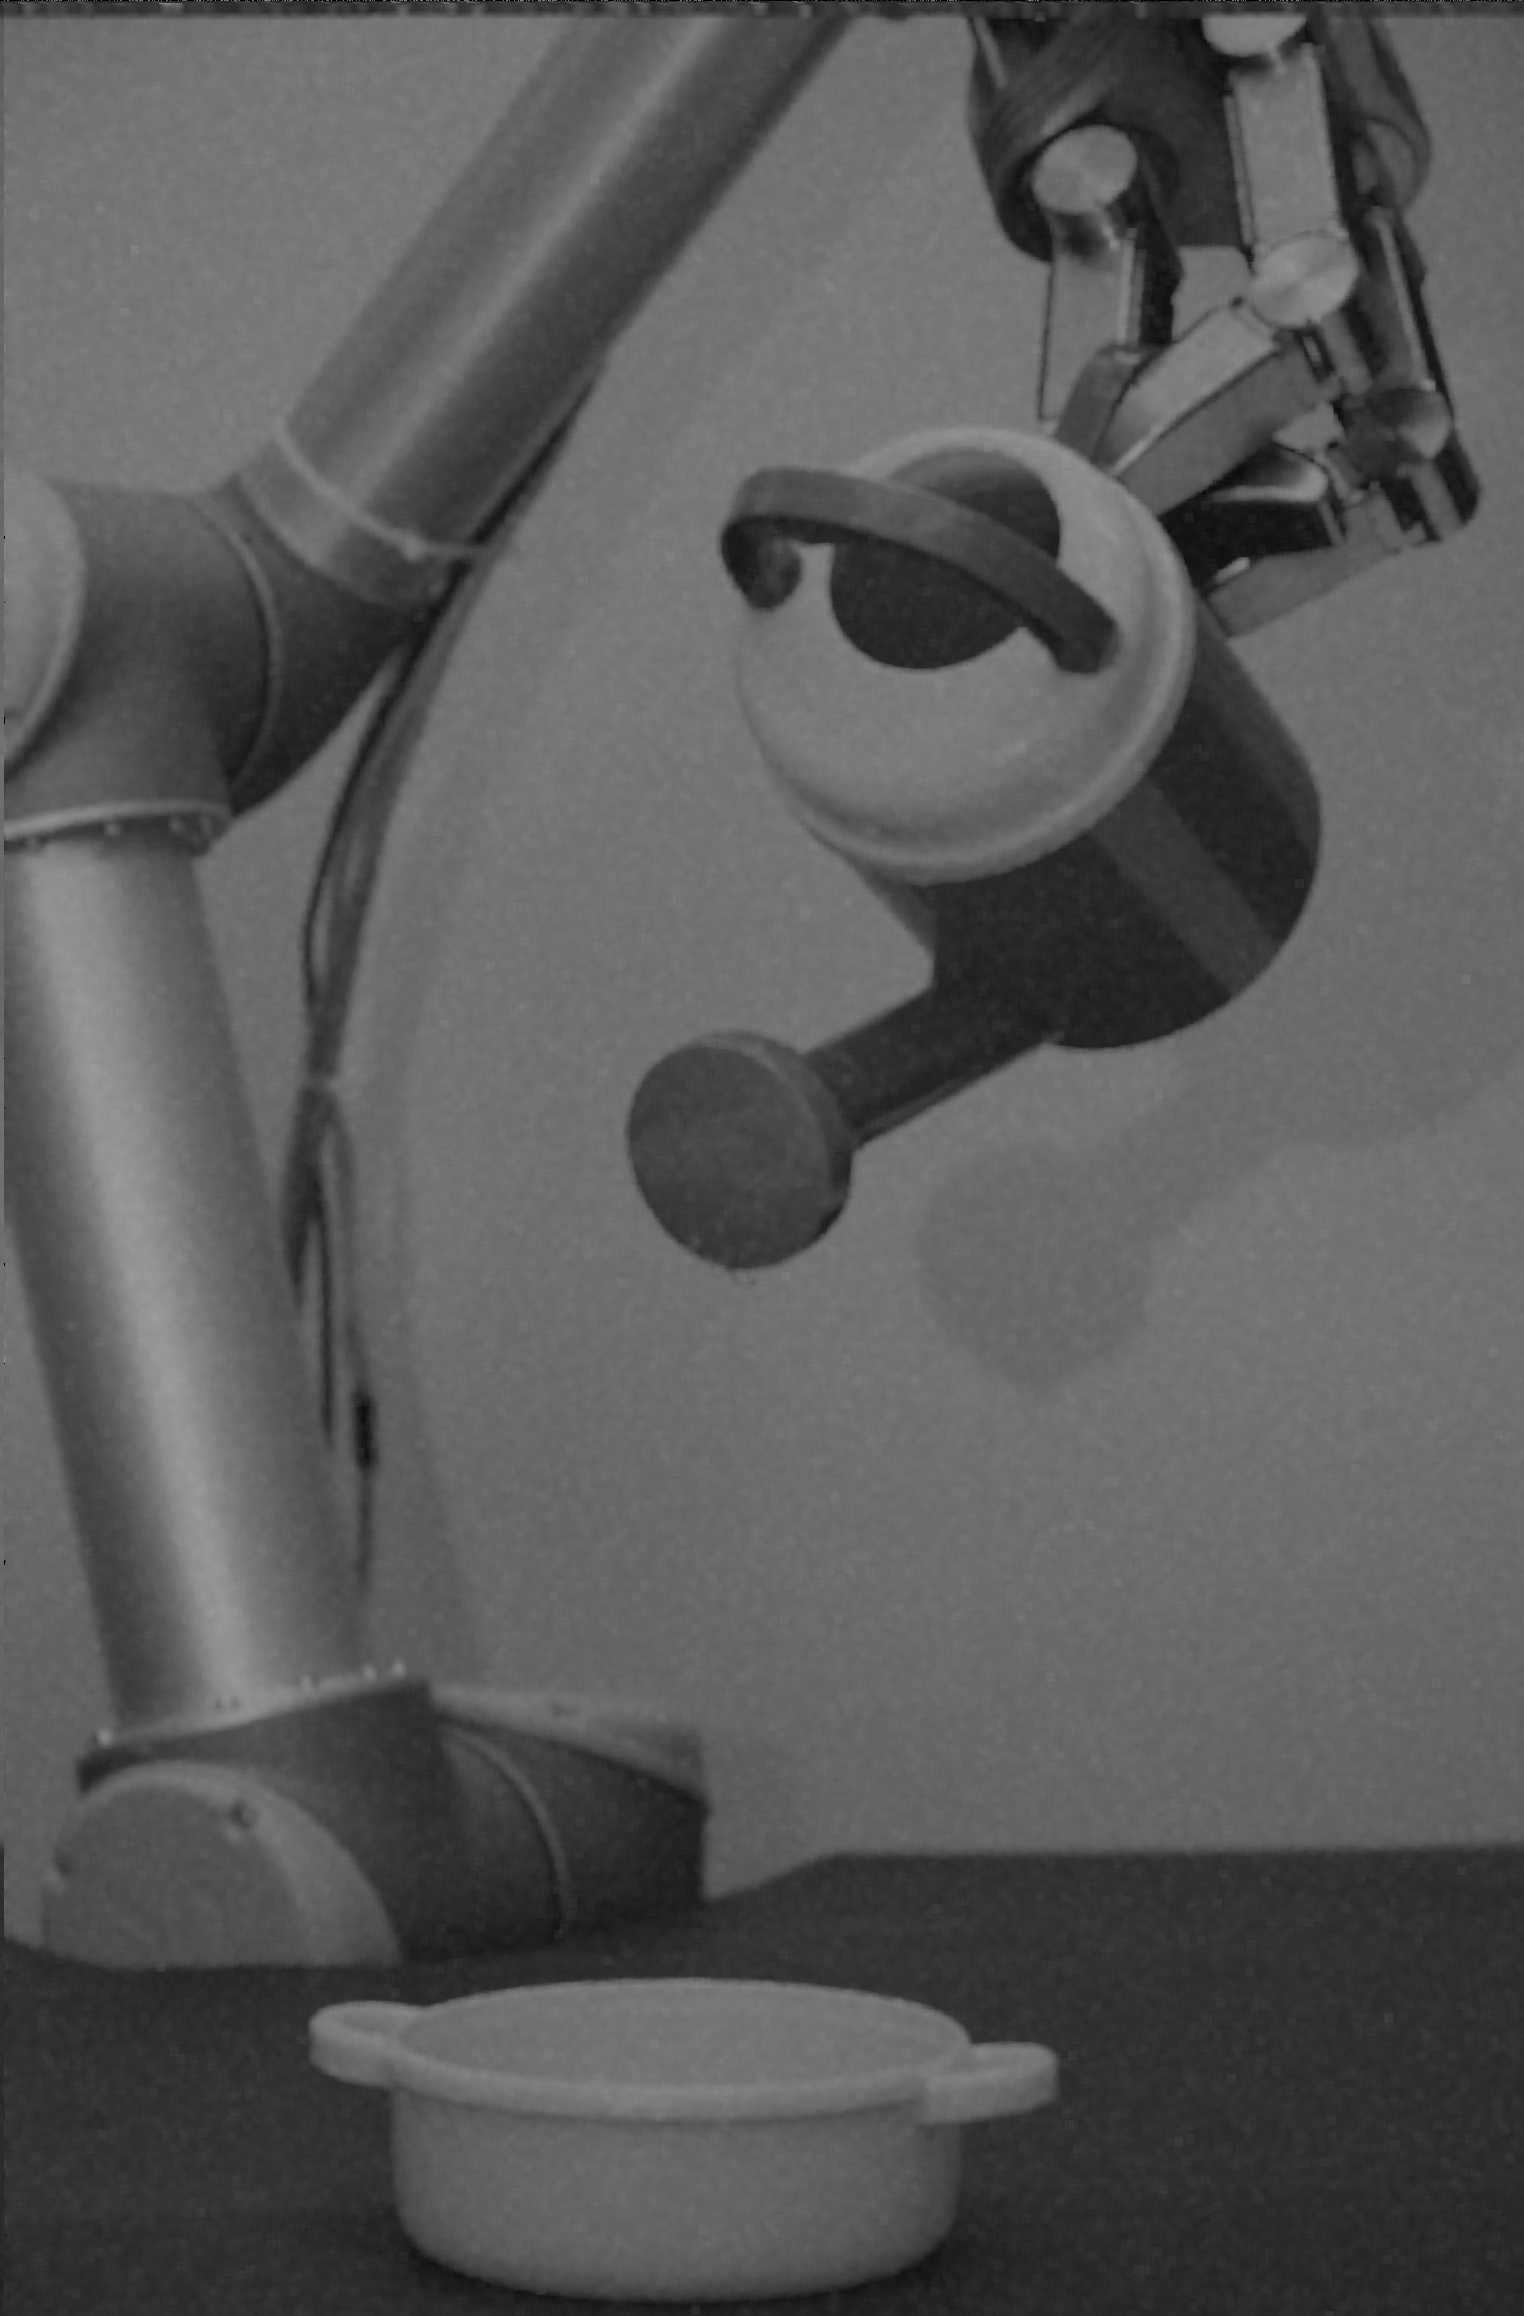
\includegraphics[width=\textwidth]{img1/img_1_gaus_9_1.png}
        \caption{Kernelsize: 9 order: 1}
         \label{fig:img1_contra9_1}
    \end{subfigure}
    \begin{subfigure}[b]{0.3\textwidth}
        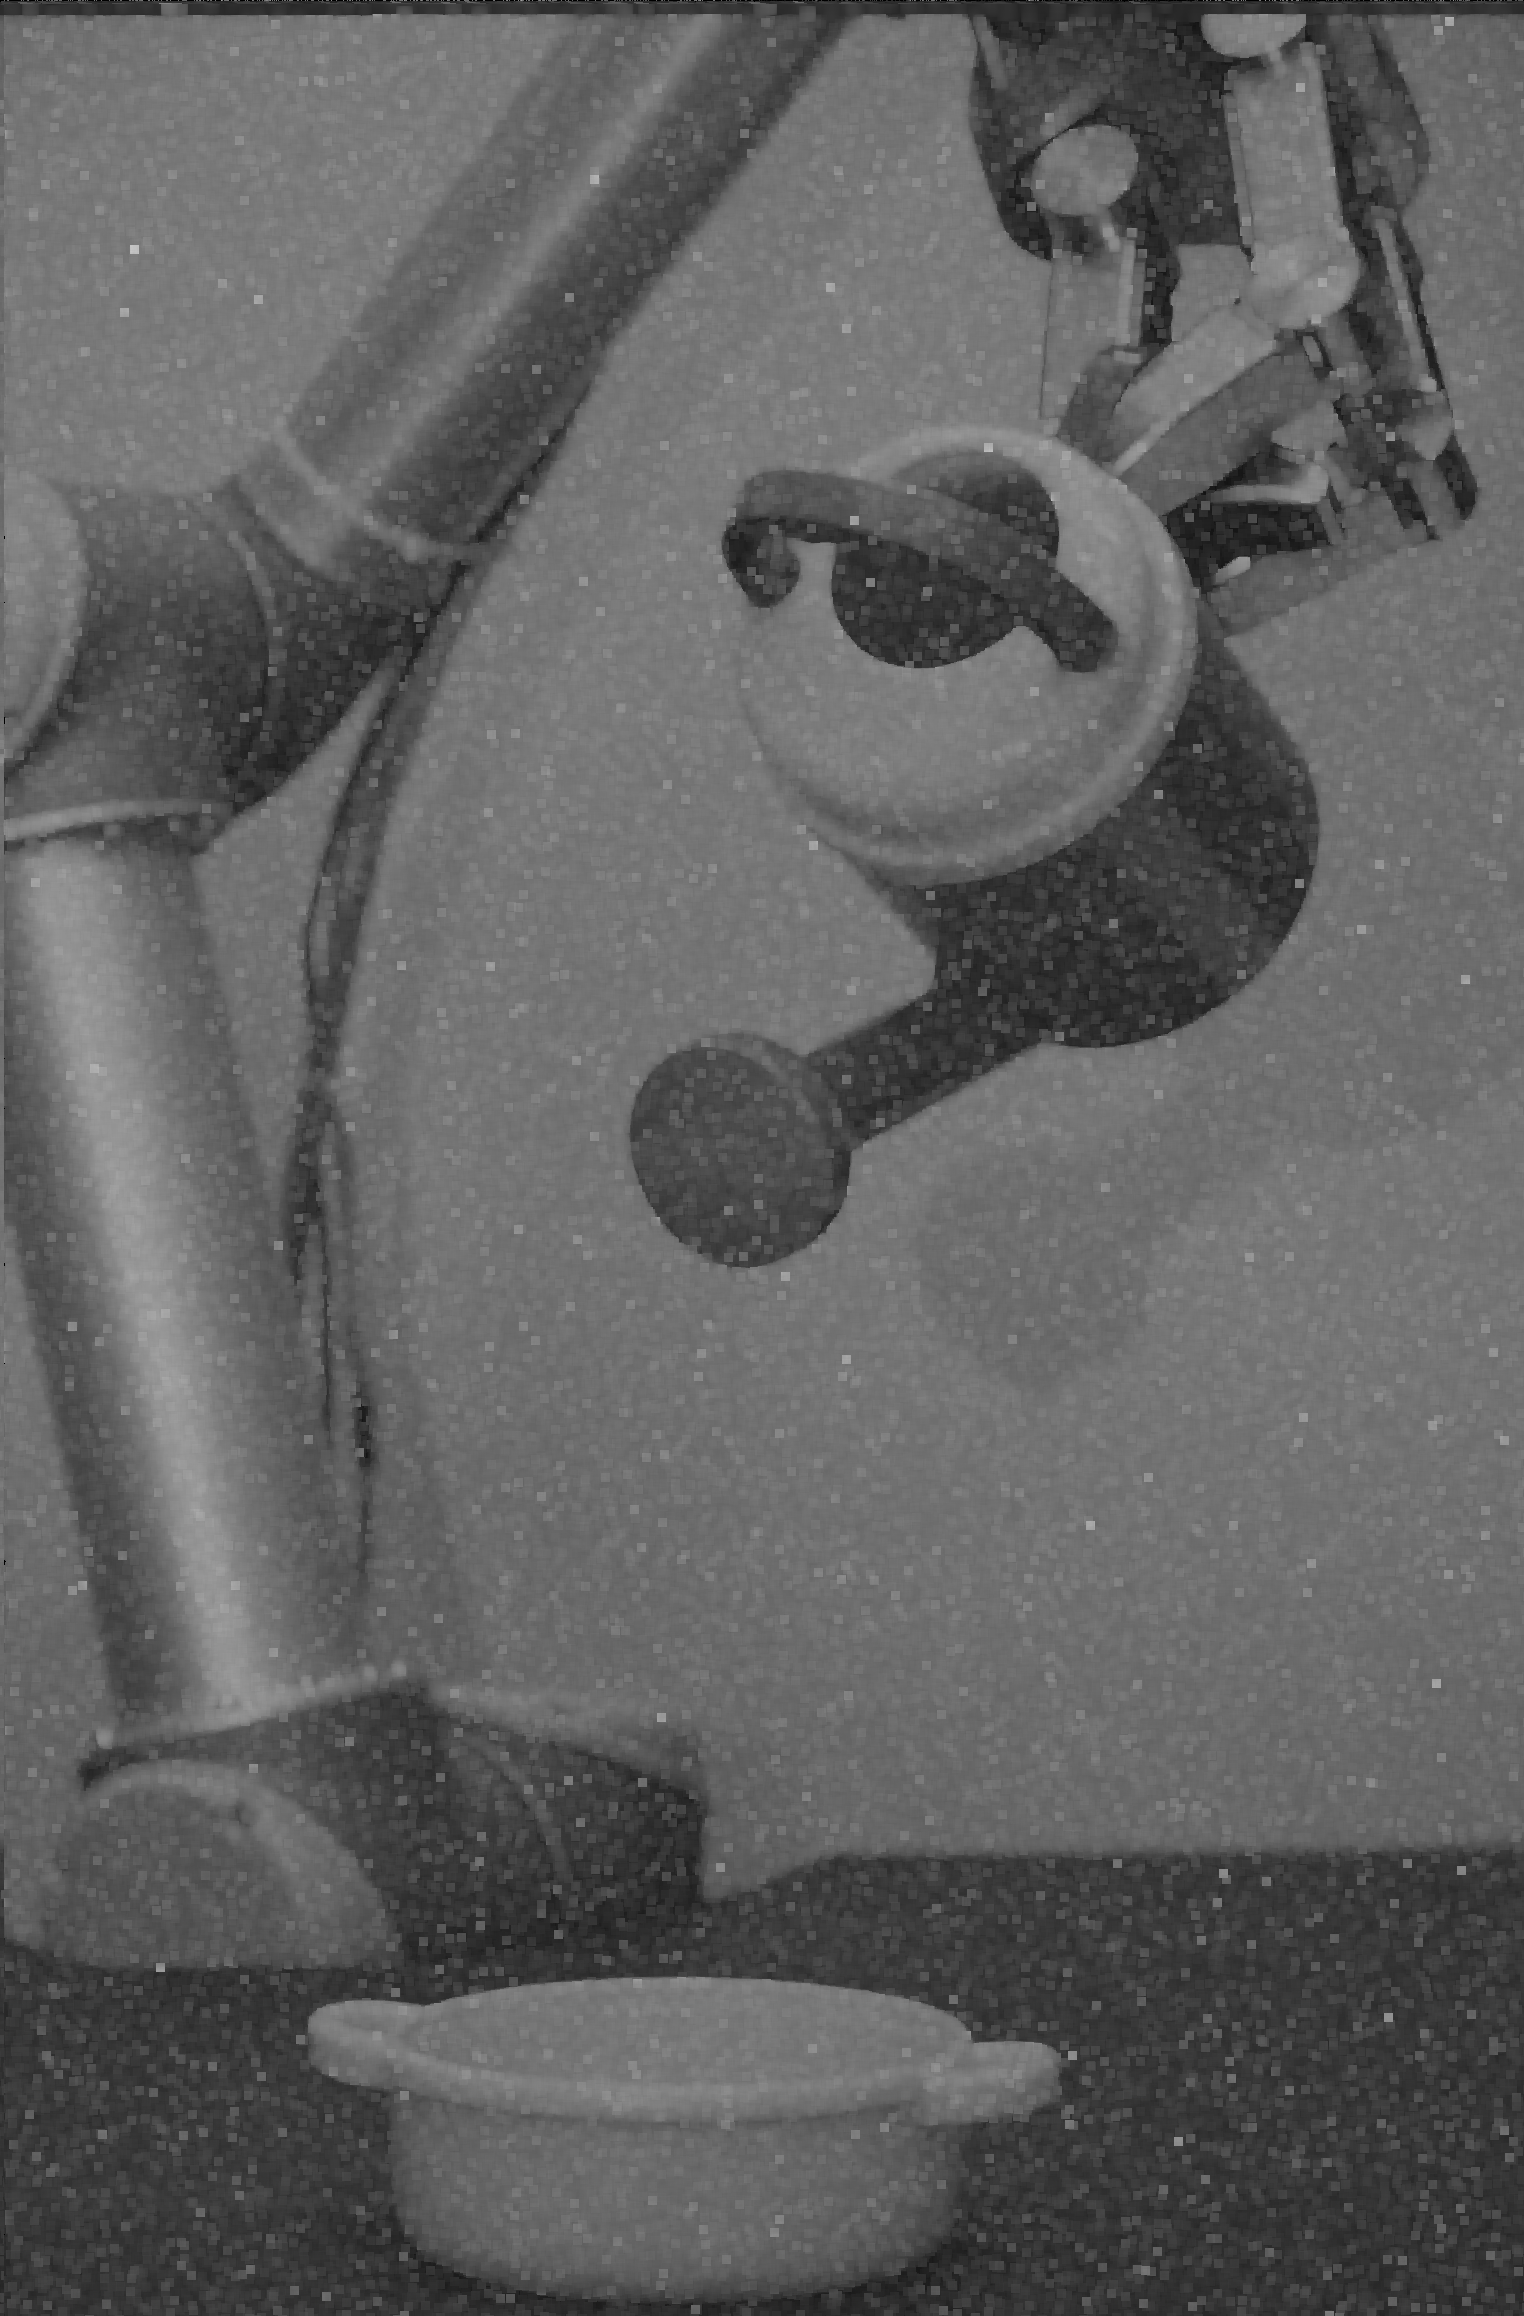
\includegraphics[width=\textwidth]{img1/img_1_gaus_9_5.png}
        \caption{Kernelsize: 9 order: 5}
         \label{fig:img1_contra9_5}
    \end{subfigure}
       \begin{subfigure}[b]{0.3\textwidth}
        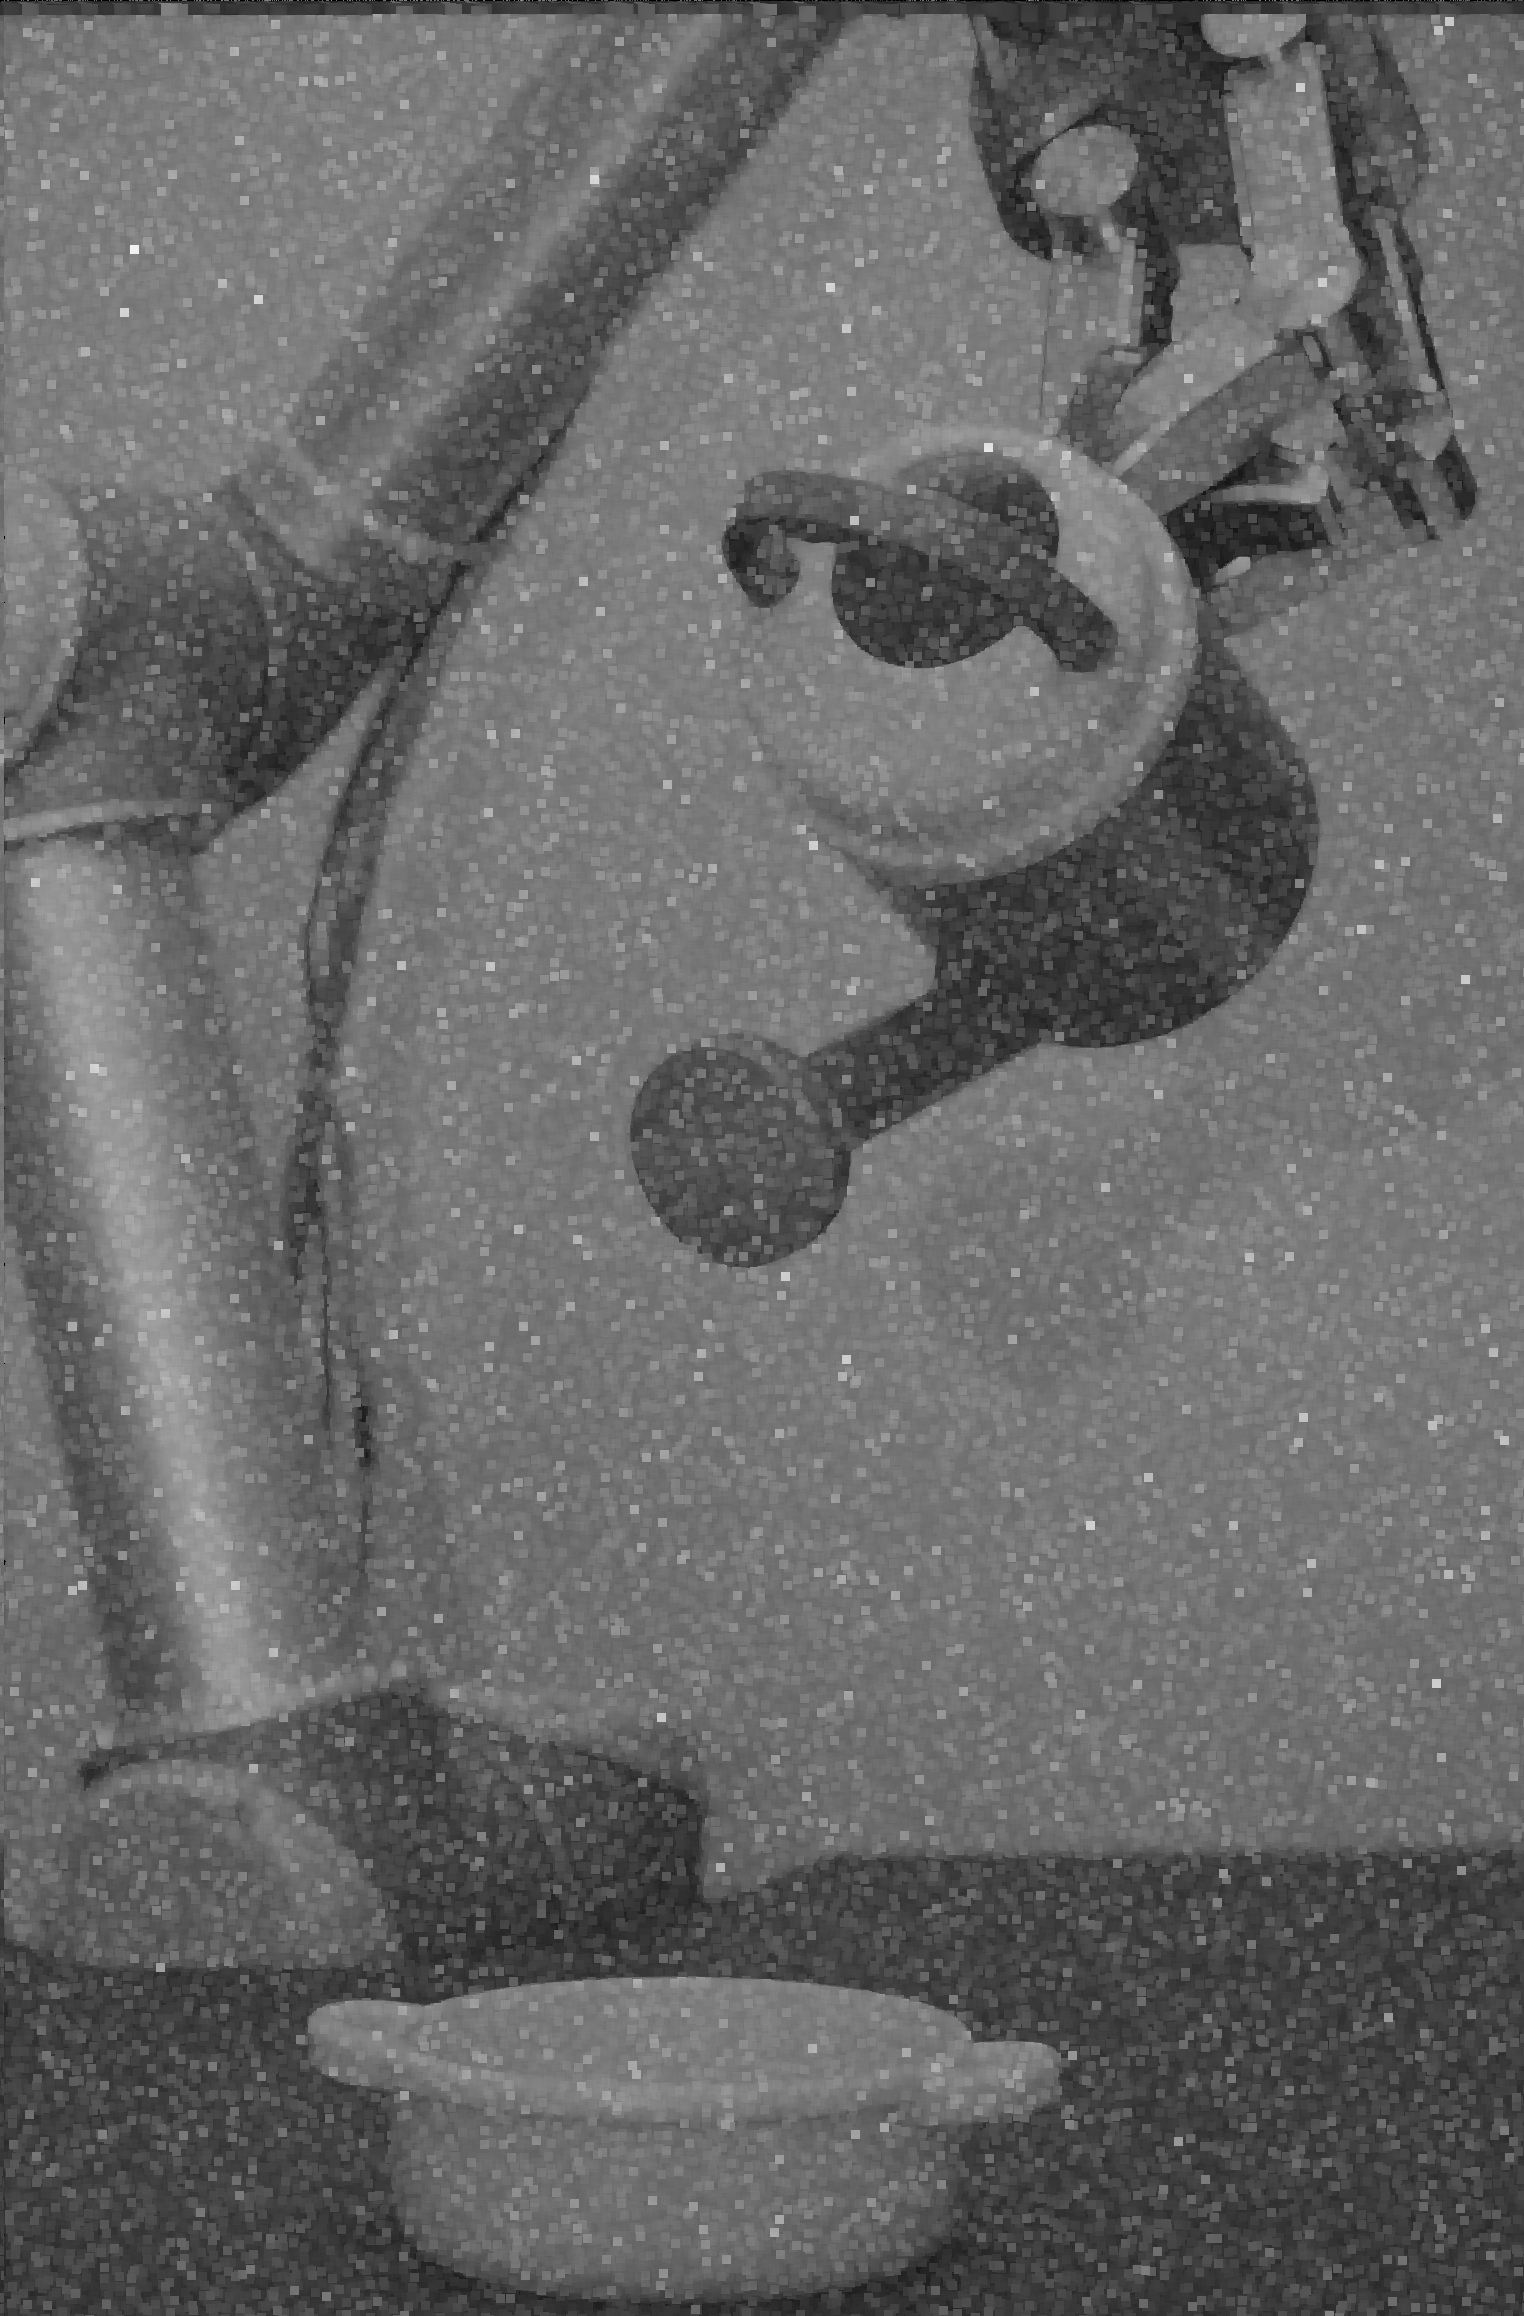
\includegraphics[width=\textwidth]{img1/img_1_gaus_9_9.png}
        \caption{Kernelsize: 9 order: 9}
         \label{fig:img1_contra9_9}
    \end{subfigure}
    
    
    
    
    
       \begin{subfigure}[b]{0.30\textwidth}
        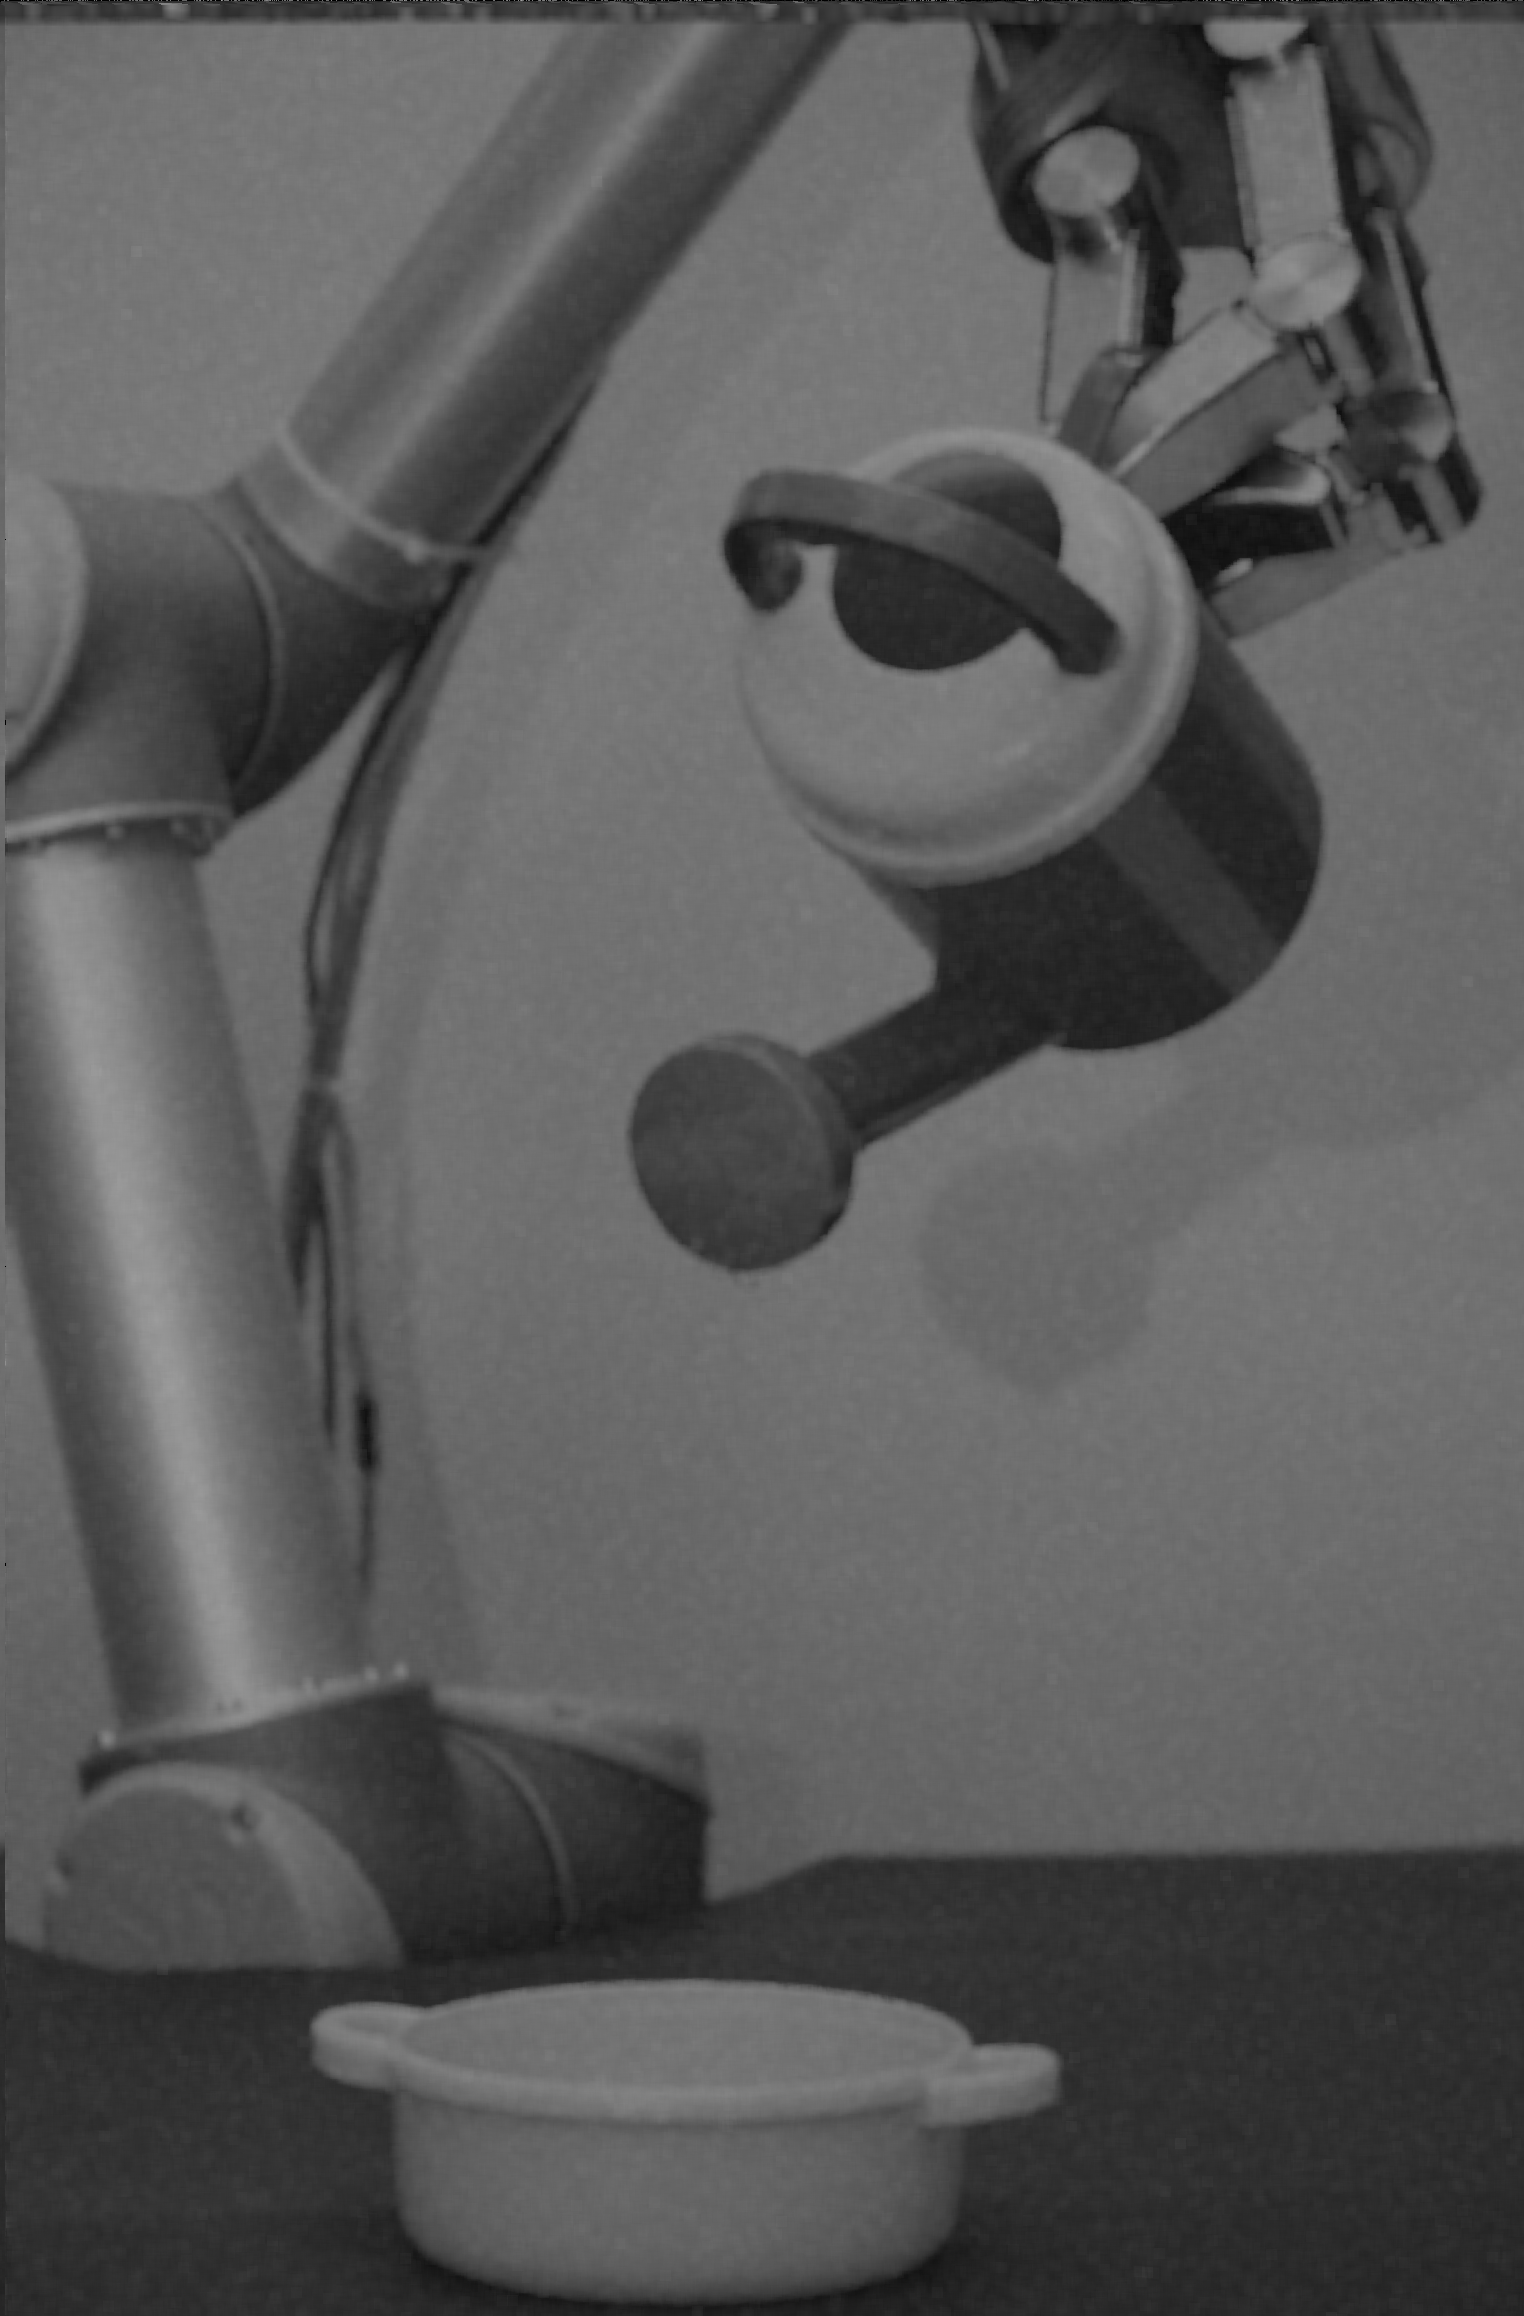
\includegraphics[width=\textwidth]{img1/img_1_gaus_11_1.png}
        \caption{Kernelsize: 11 order: 1}
         \label{fig:img1_contra11_1}
    \end{subfigure}
    \begin{subfigure}[b]{0.30\textwidth}
        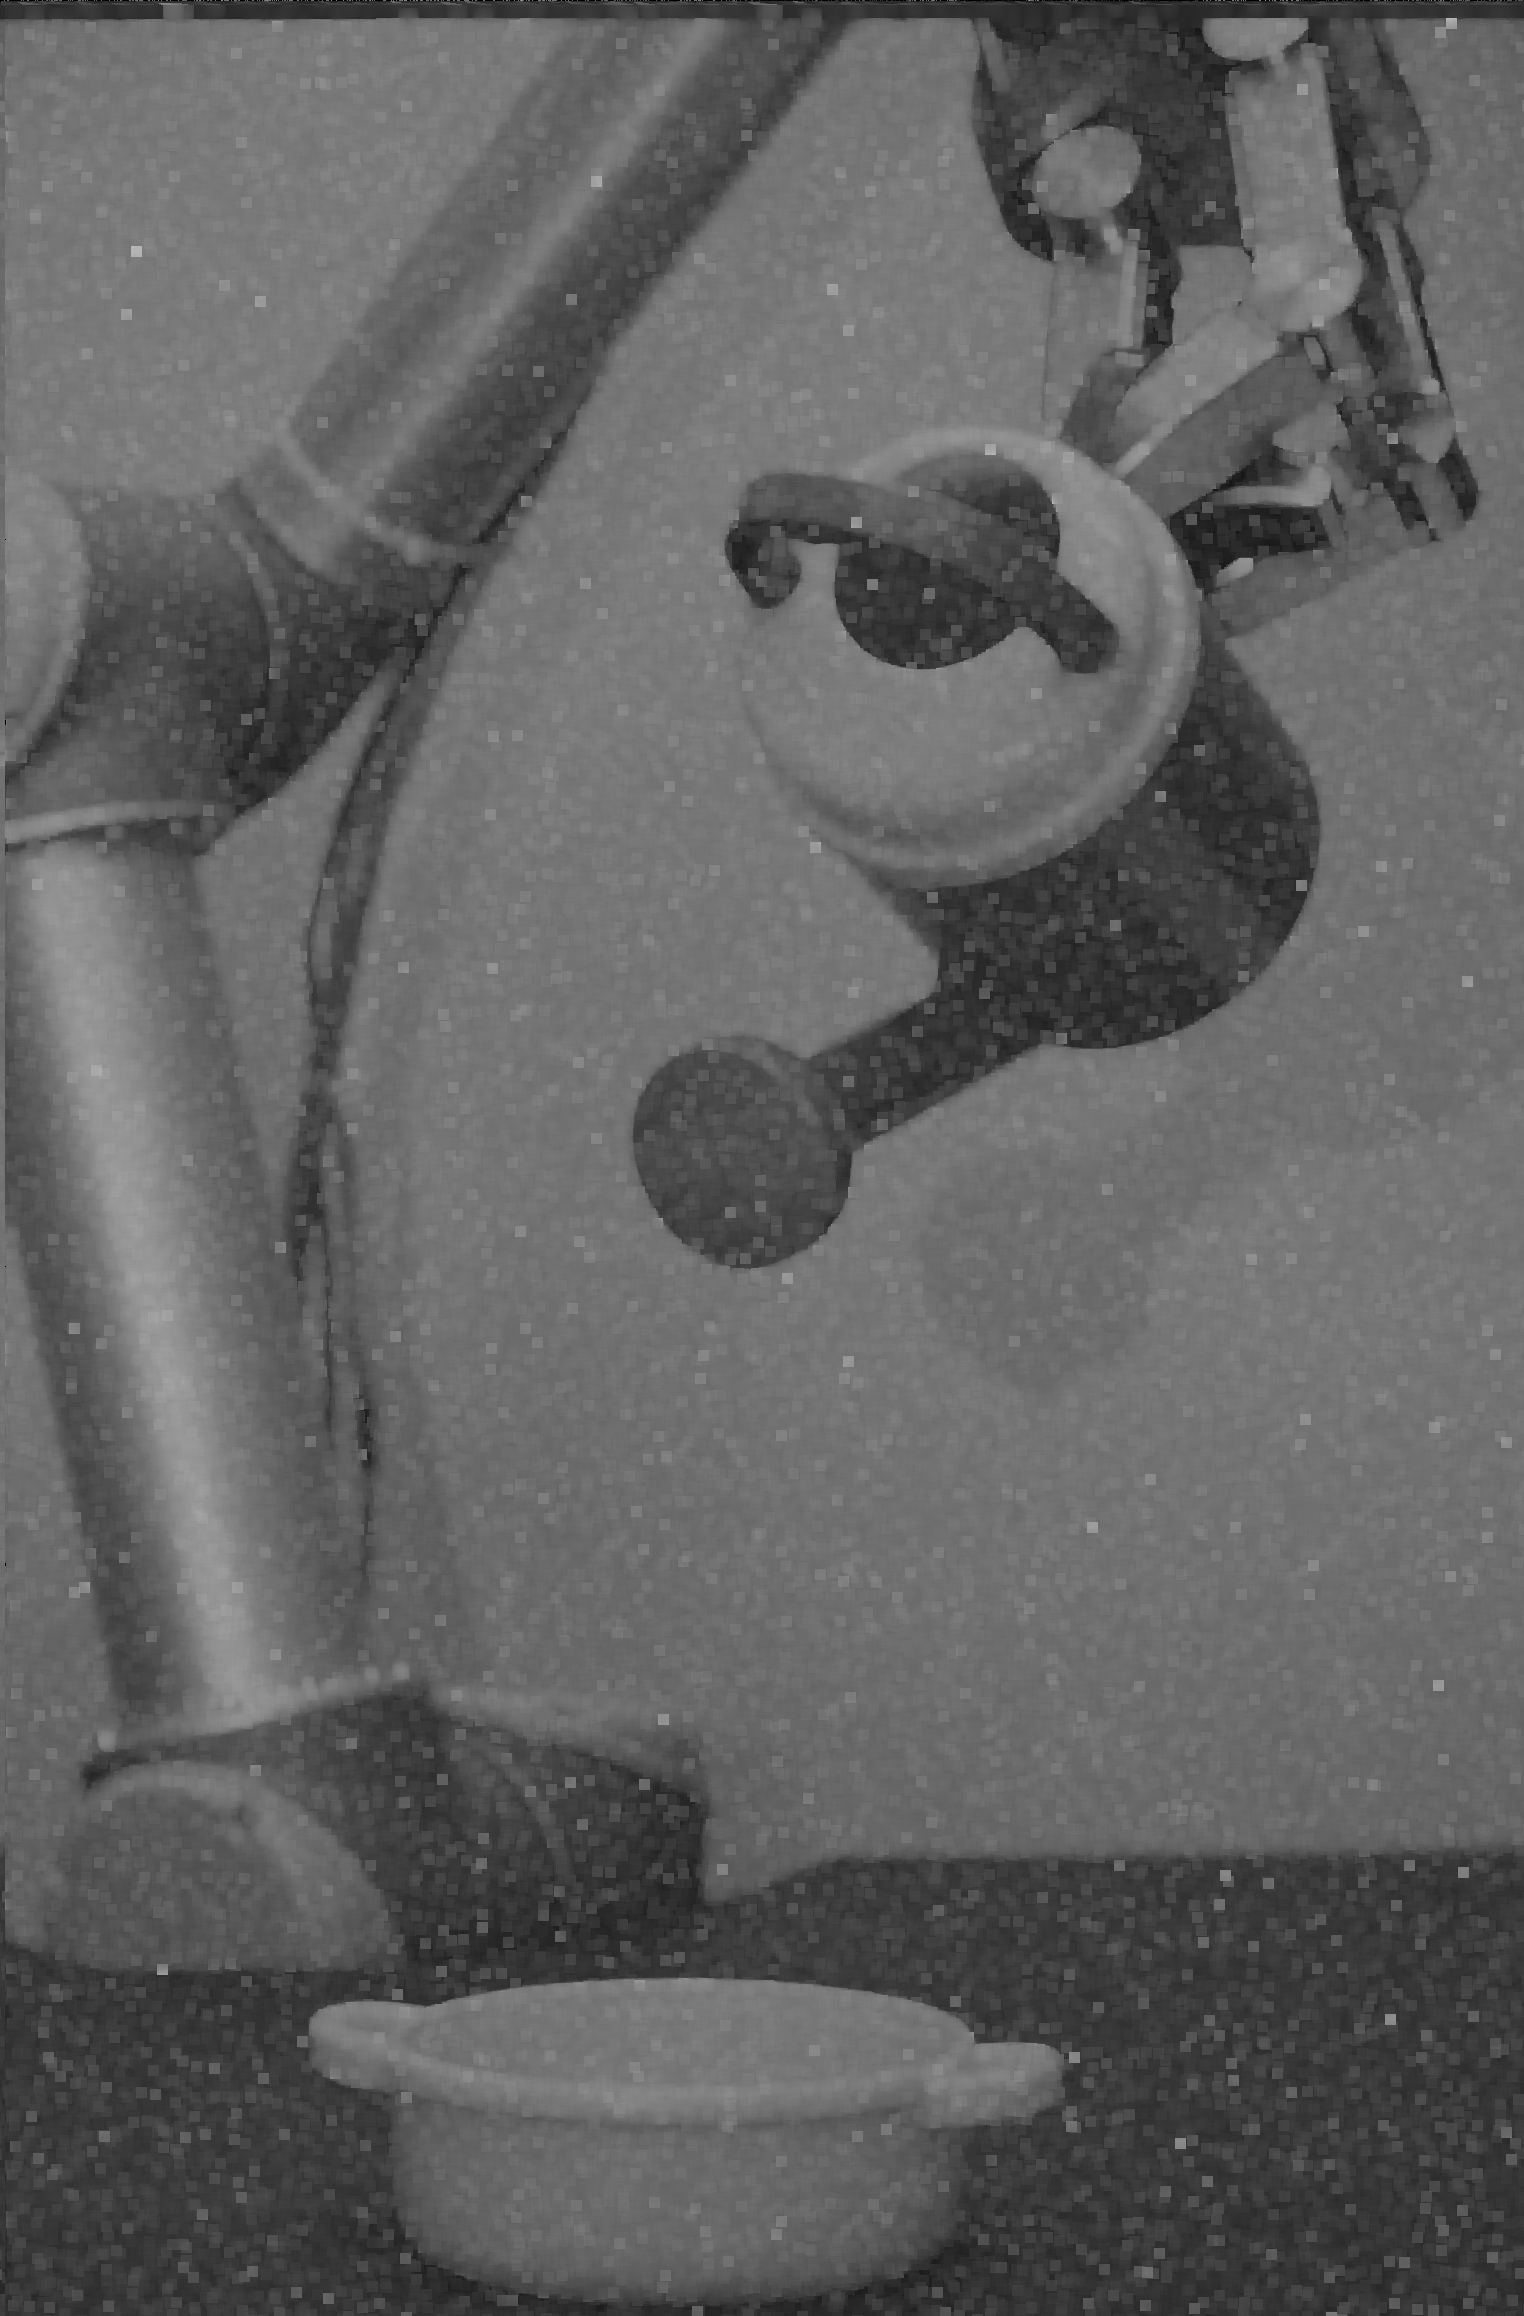
\includegraphics[width=\textwidth]{img1/img_1_gaus_11_5.png}
        \caption{Kernelsize: 11 order: 5}
         \label{fig:img1_contra11_5}
    \end{subfigure}
       \begin{subfigure}[b]{0.30\textwidth}
        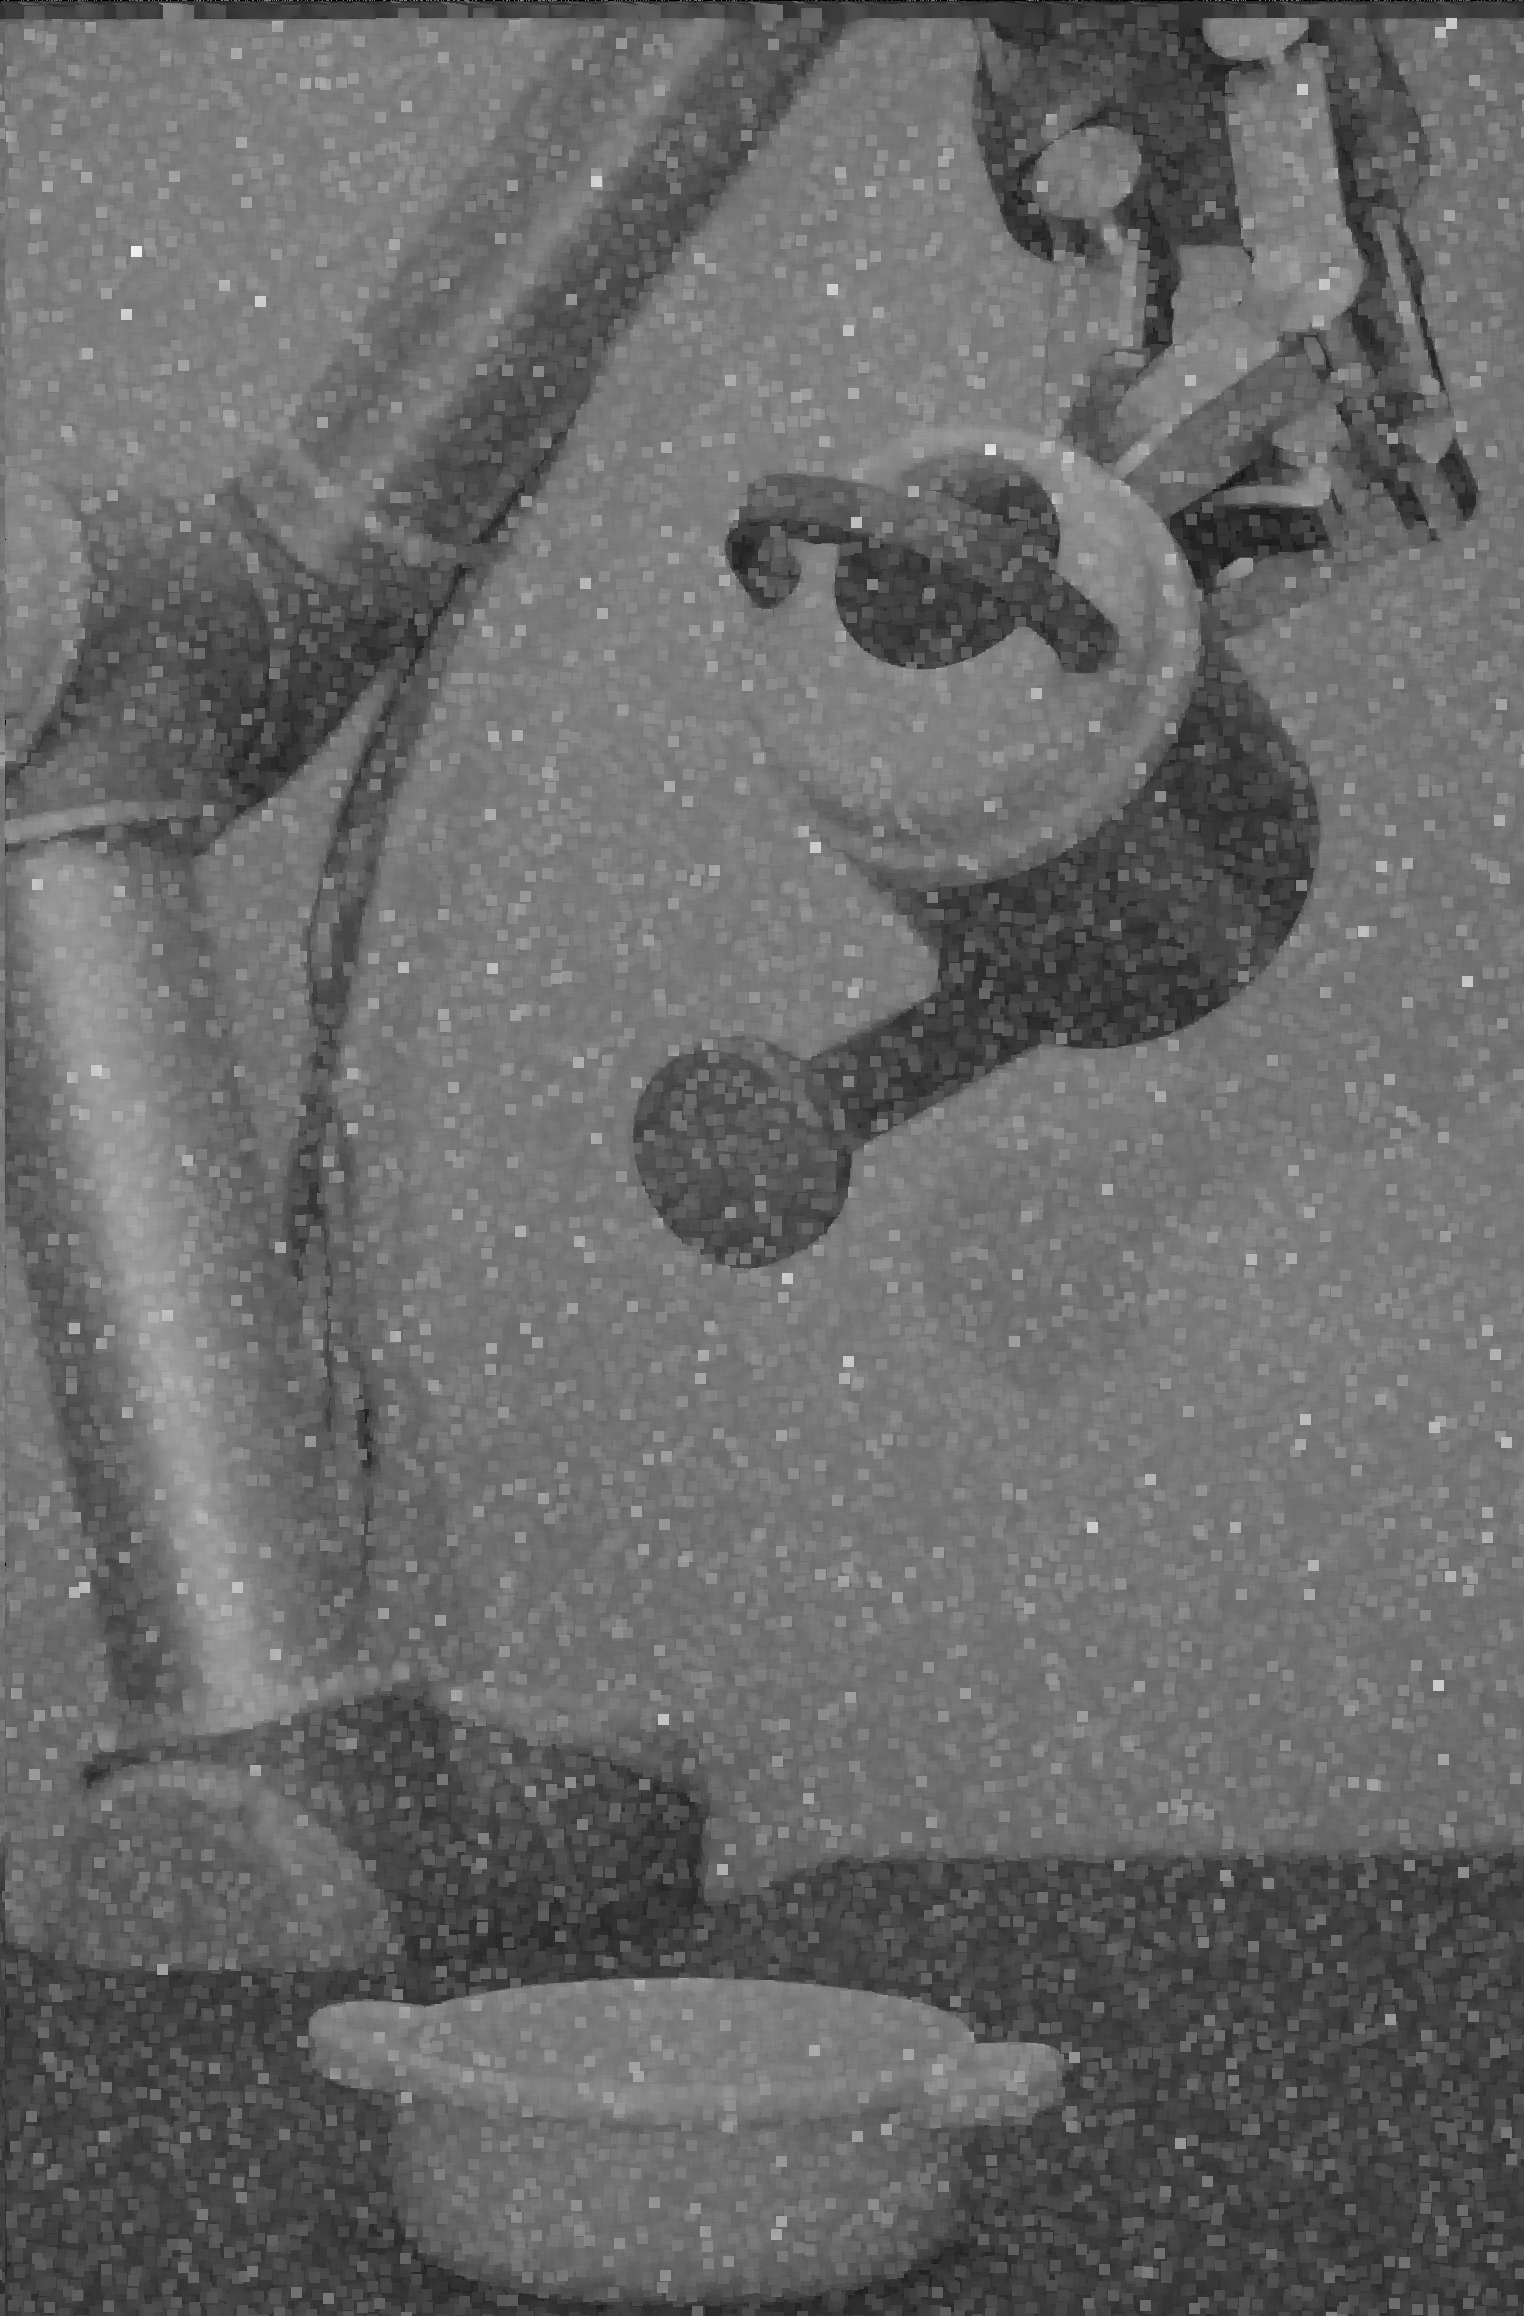
\includegraphics[width=\textwidth]{img1/img_1_gaus_11_9.png}
        \caption{Kernelsize: 11 order: 9}
		 \label{fig:img1_contra11_9}
    \end{subfigure}
    \caption{Contraharmonic mean filter applied on Figure \ref{fig:img1_src} with different kernel sizes and orders}
    \label{fig:img1_contra}
\end{figure}

By visual inspection it can be seen that the Contraharmonic mean filter has removed most of the black pepper noise which was visible in Figure \ref{fig:img1_src}. As the kernel and order size increases it can be seen that output image becomes more blurred and more of the pepper noise  get removed, but also introduces more  salt noise.  Therefore was order sizes above one deemed unuseful .   The only filter which was capable of removing most of the pepper noise, and still keep the image minimally blurred is the output from the filter with an kernelsize of 5, and order 1 Figure \ref{fig:img1_contra5_1}. Which was used for further processing. \\

The image is still a bit dark compared to the original image, to reduce its poor contrast was a method called contrast stretching implemented and applied to that image.  This method tries to expand the range of intensity levels the image contains, such that the full intensity range of the image will be used. \\
\todo{ciite http://www.tutorialspoint.com/dip/Histogram\_Stretching.htm}\\

Compared to histogram equalization is this method more subtle, and tries to keep the original histogram shape, where an equalization  will try to equalize all bins in a histogram, and thus radically distort the image, and change the histogram from its original appereance.\\



The Contrast stretching is  done by modifying each pixel in the image using Equation \ref{eq:contrast_eq}

\begin{equation}
\hat{f}(x,y) = \frac{g(x,y) - minP}{maxP - minP} \cdot 2^{bpp }-1
\label{eq:contrast_eq}
\end{equation}
  
$\hat{f}$ is the new image,  $(x,y)$ is  a pixel position, $g$ is the original image, $minP$ is the lowest pixel value in image $g$, $maxP$ is the max pixel value in image $g$ and$ bpp$, is the bit depth of the image. 

The result of using this method can be seen here. 

\begin{figure}[H]
\centering
 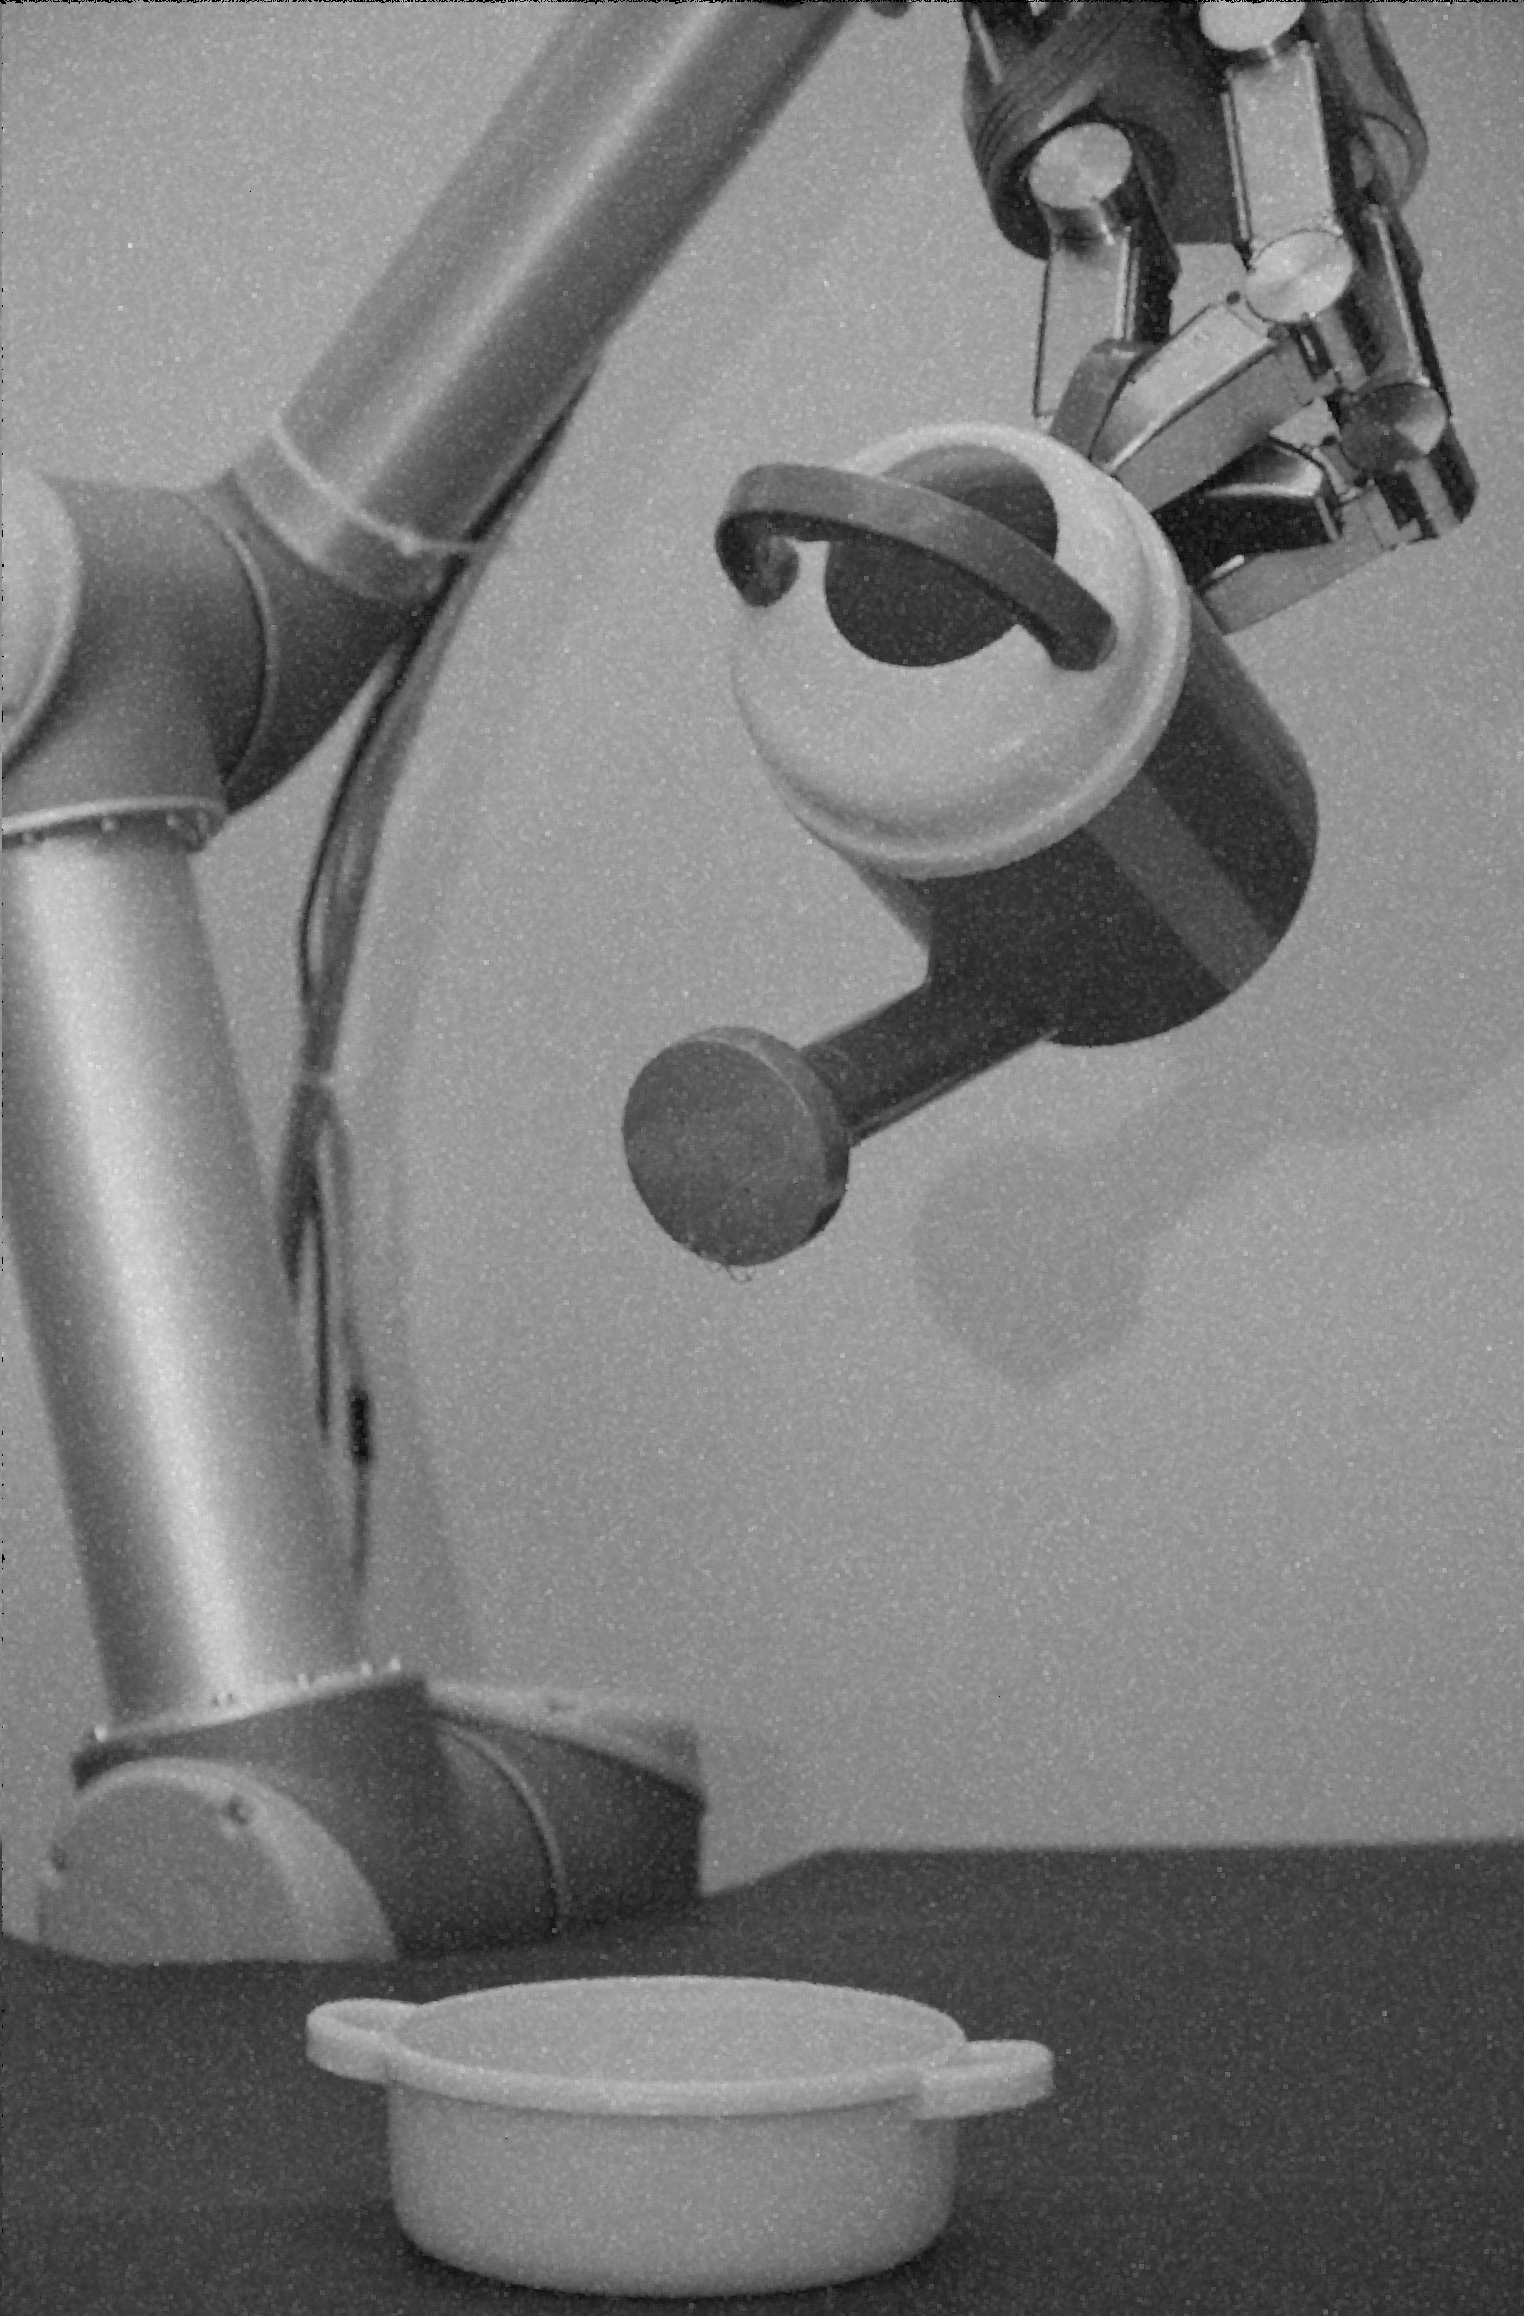
\includegraphics[width=0.30\textwidth]{img1/img_1_gaus_5_1_constrast_strech.png}
        \caption{Contrast streched image}
         \label{fig:img1_contra11_1}
\end{figure}

At this point it was determined that image has been restored enough to resemble the original image. 

\begin{figure}[H]
   \begin{subfigure}[b]{0.24\textwidth}
        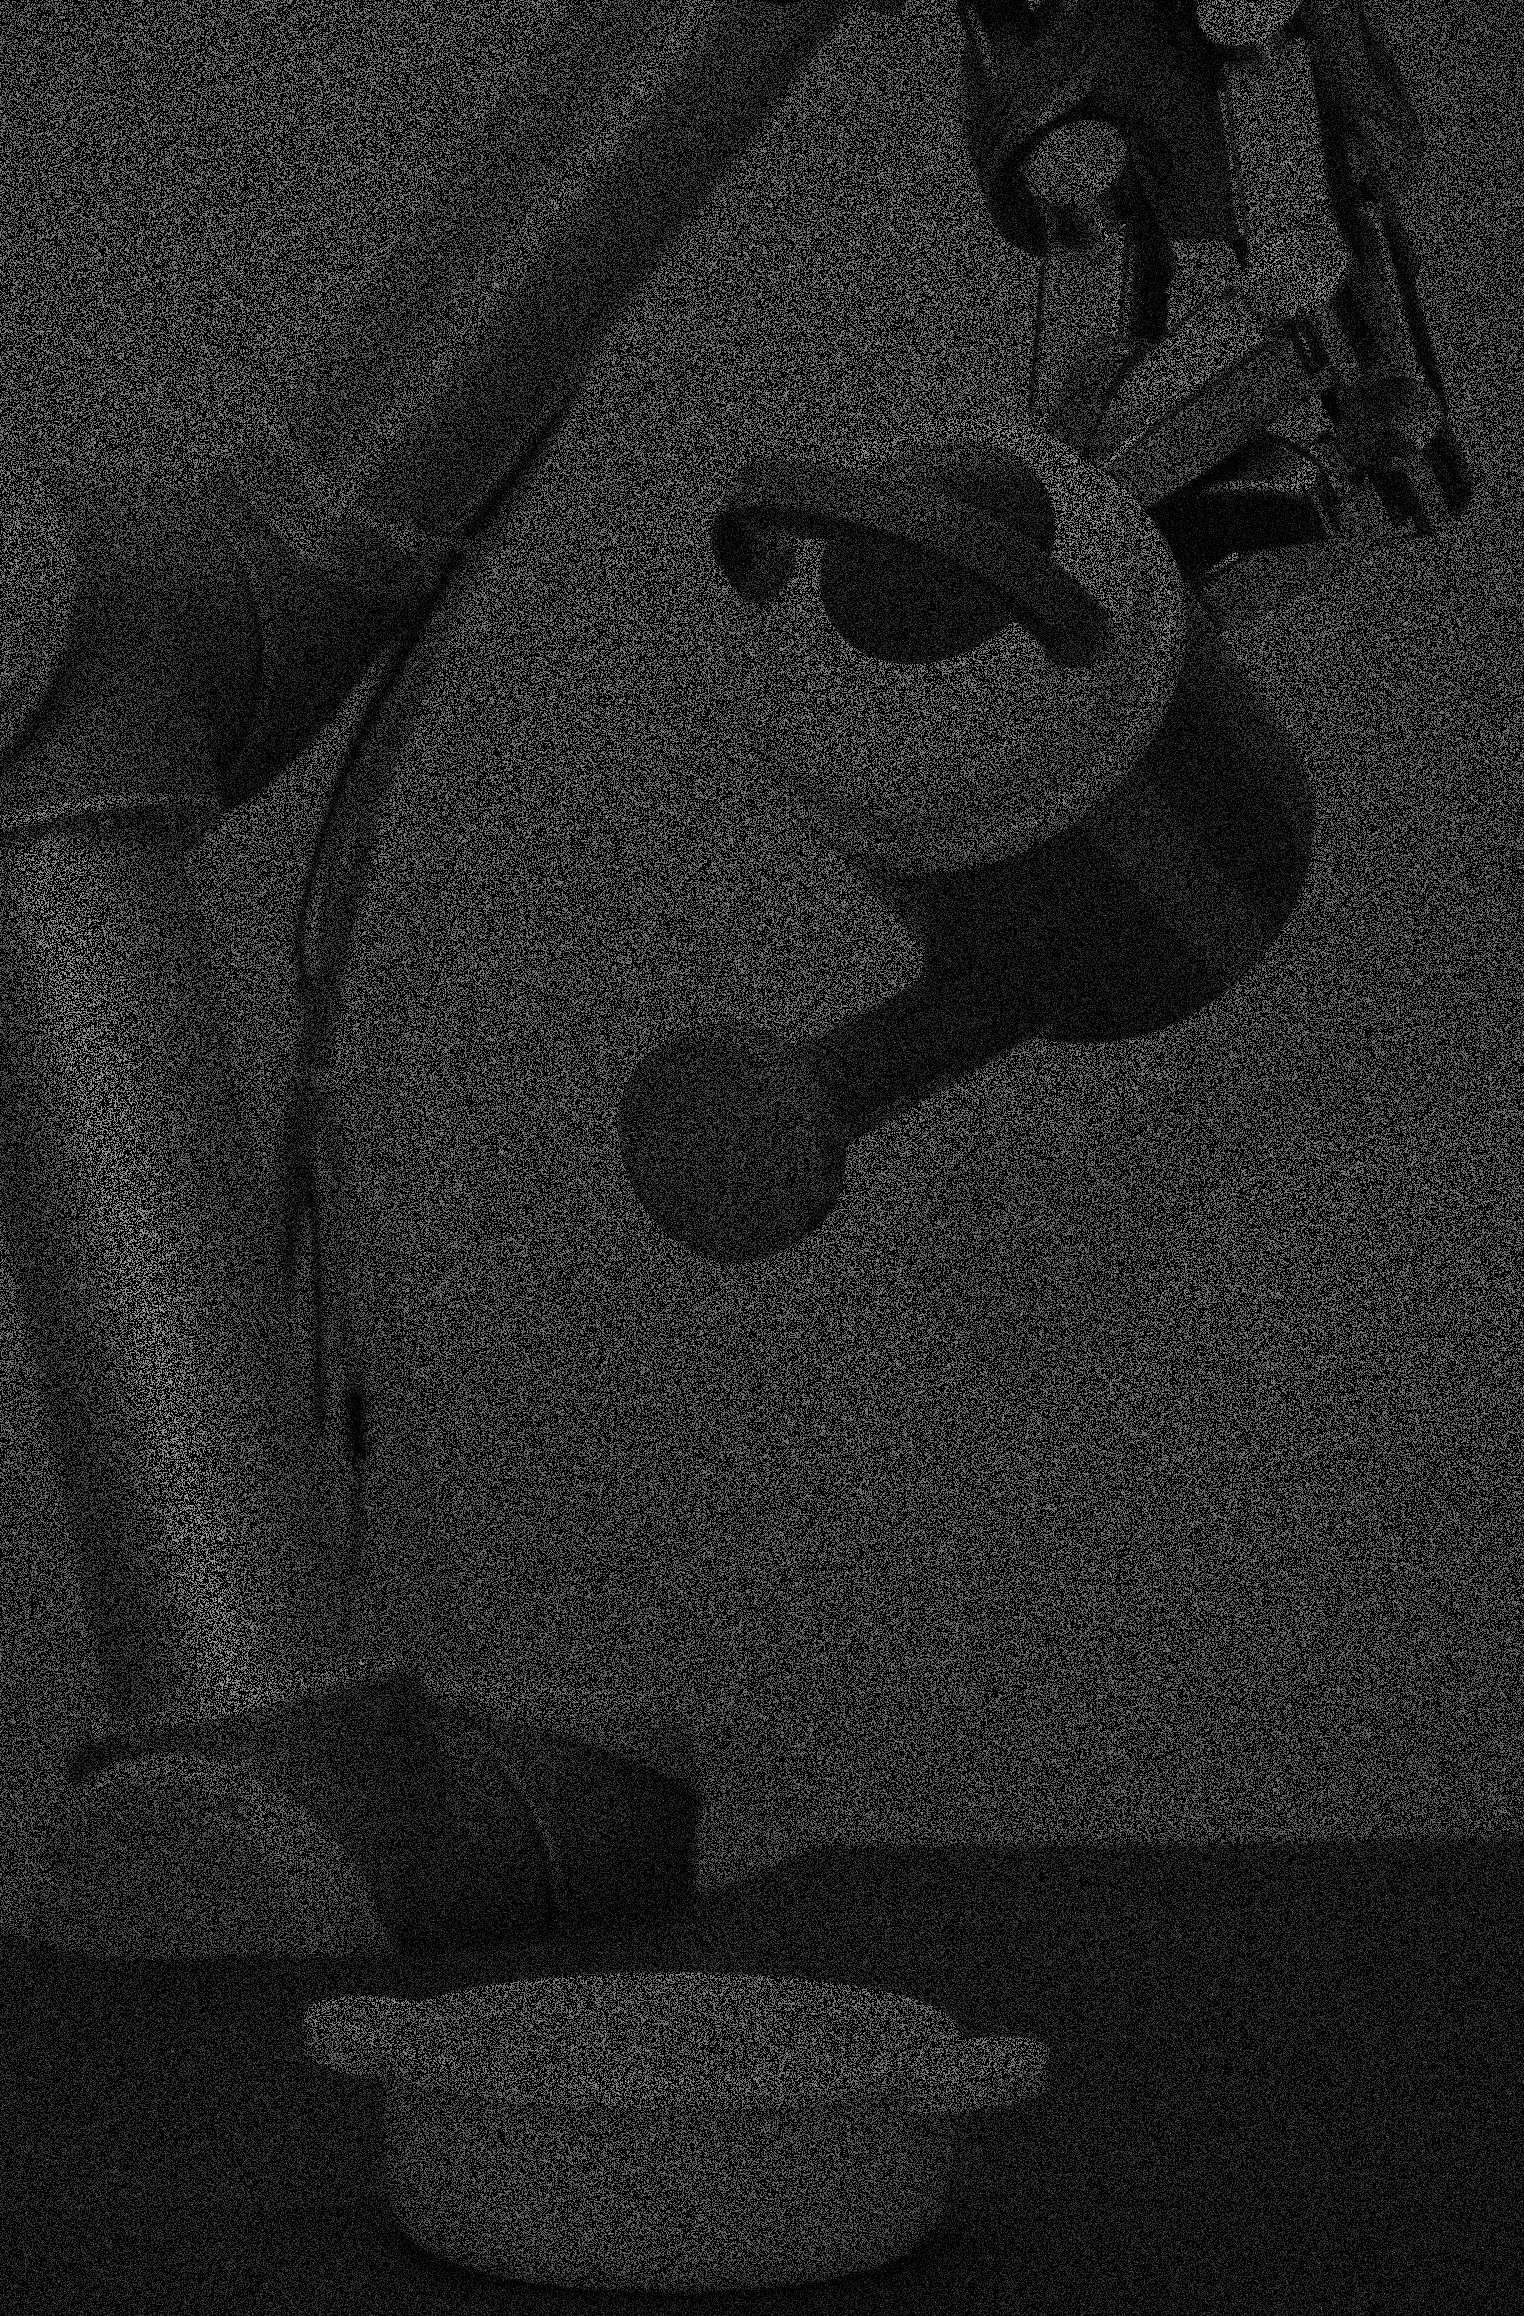
\includegraphics[width=\textwidth]{img1/Image1.png}
        \caption{Image with noise}
         %\label{fig:img1_contra11_1}
    \end{subfigure}
    \begin{subfigure}[b]{0.24\textwidth}
        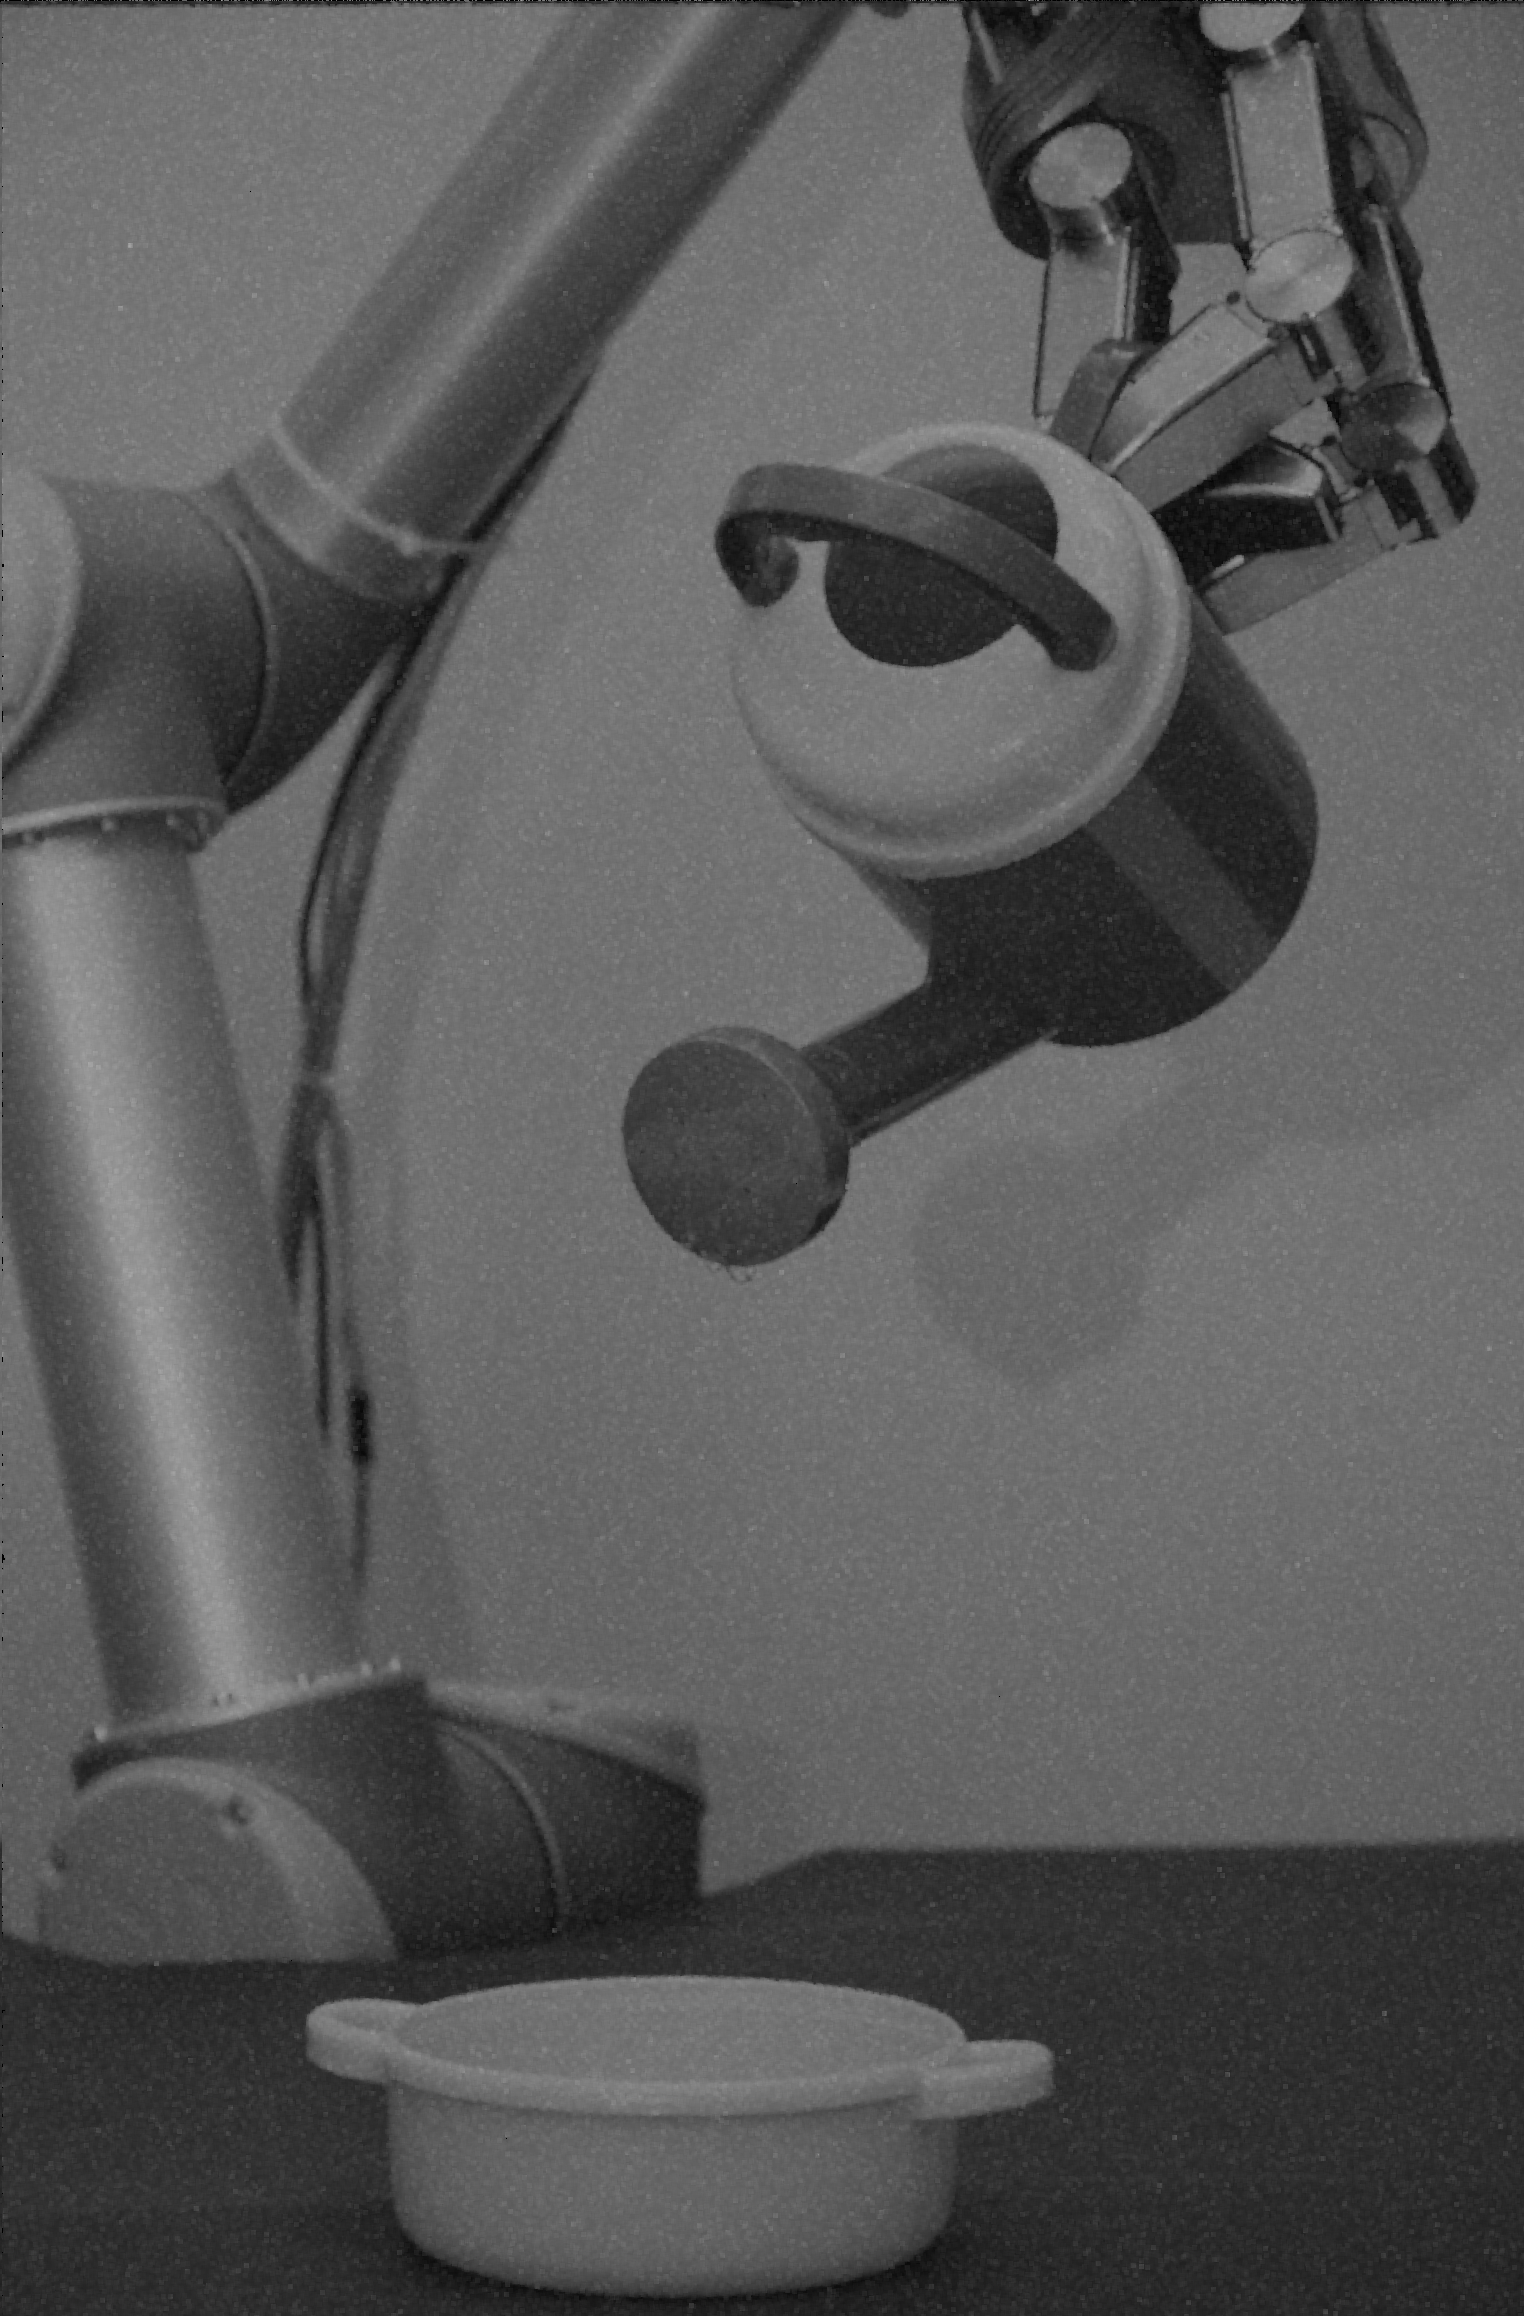
\includegraphics[width=\textwidth]{img1/img_1_gaus_5_1.png}
        \caption{Contra harmonic mean filter applied}
         %\label{fig:img1_contra11_5}
    \end{subfigure}  
       \begin{subfigure}[b]{0.24\textwidth}
        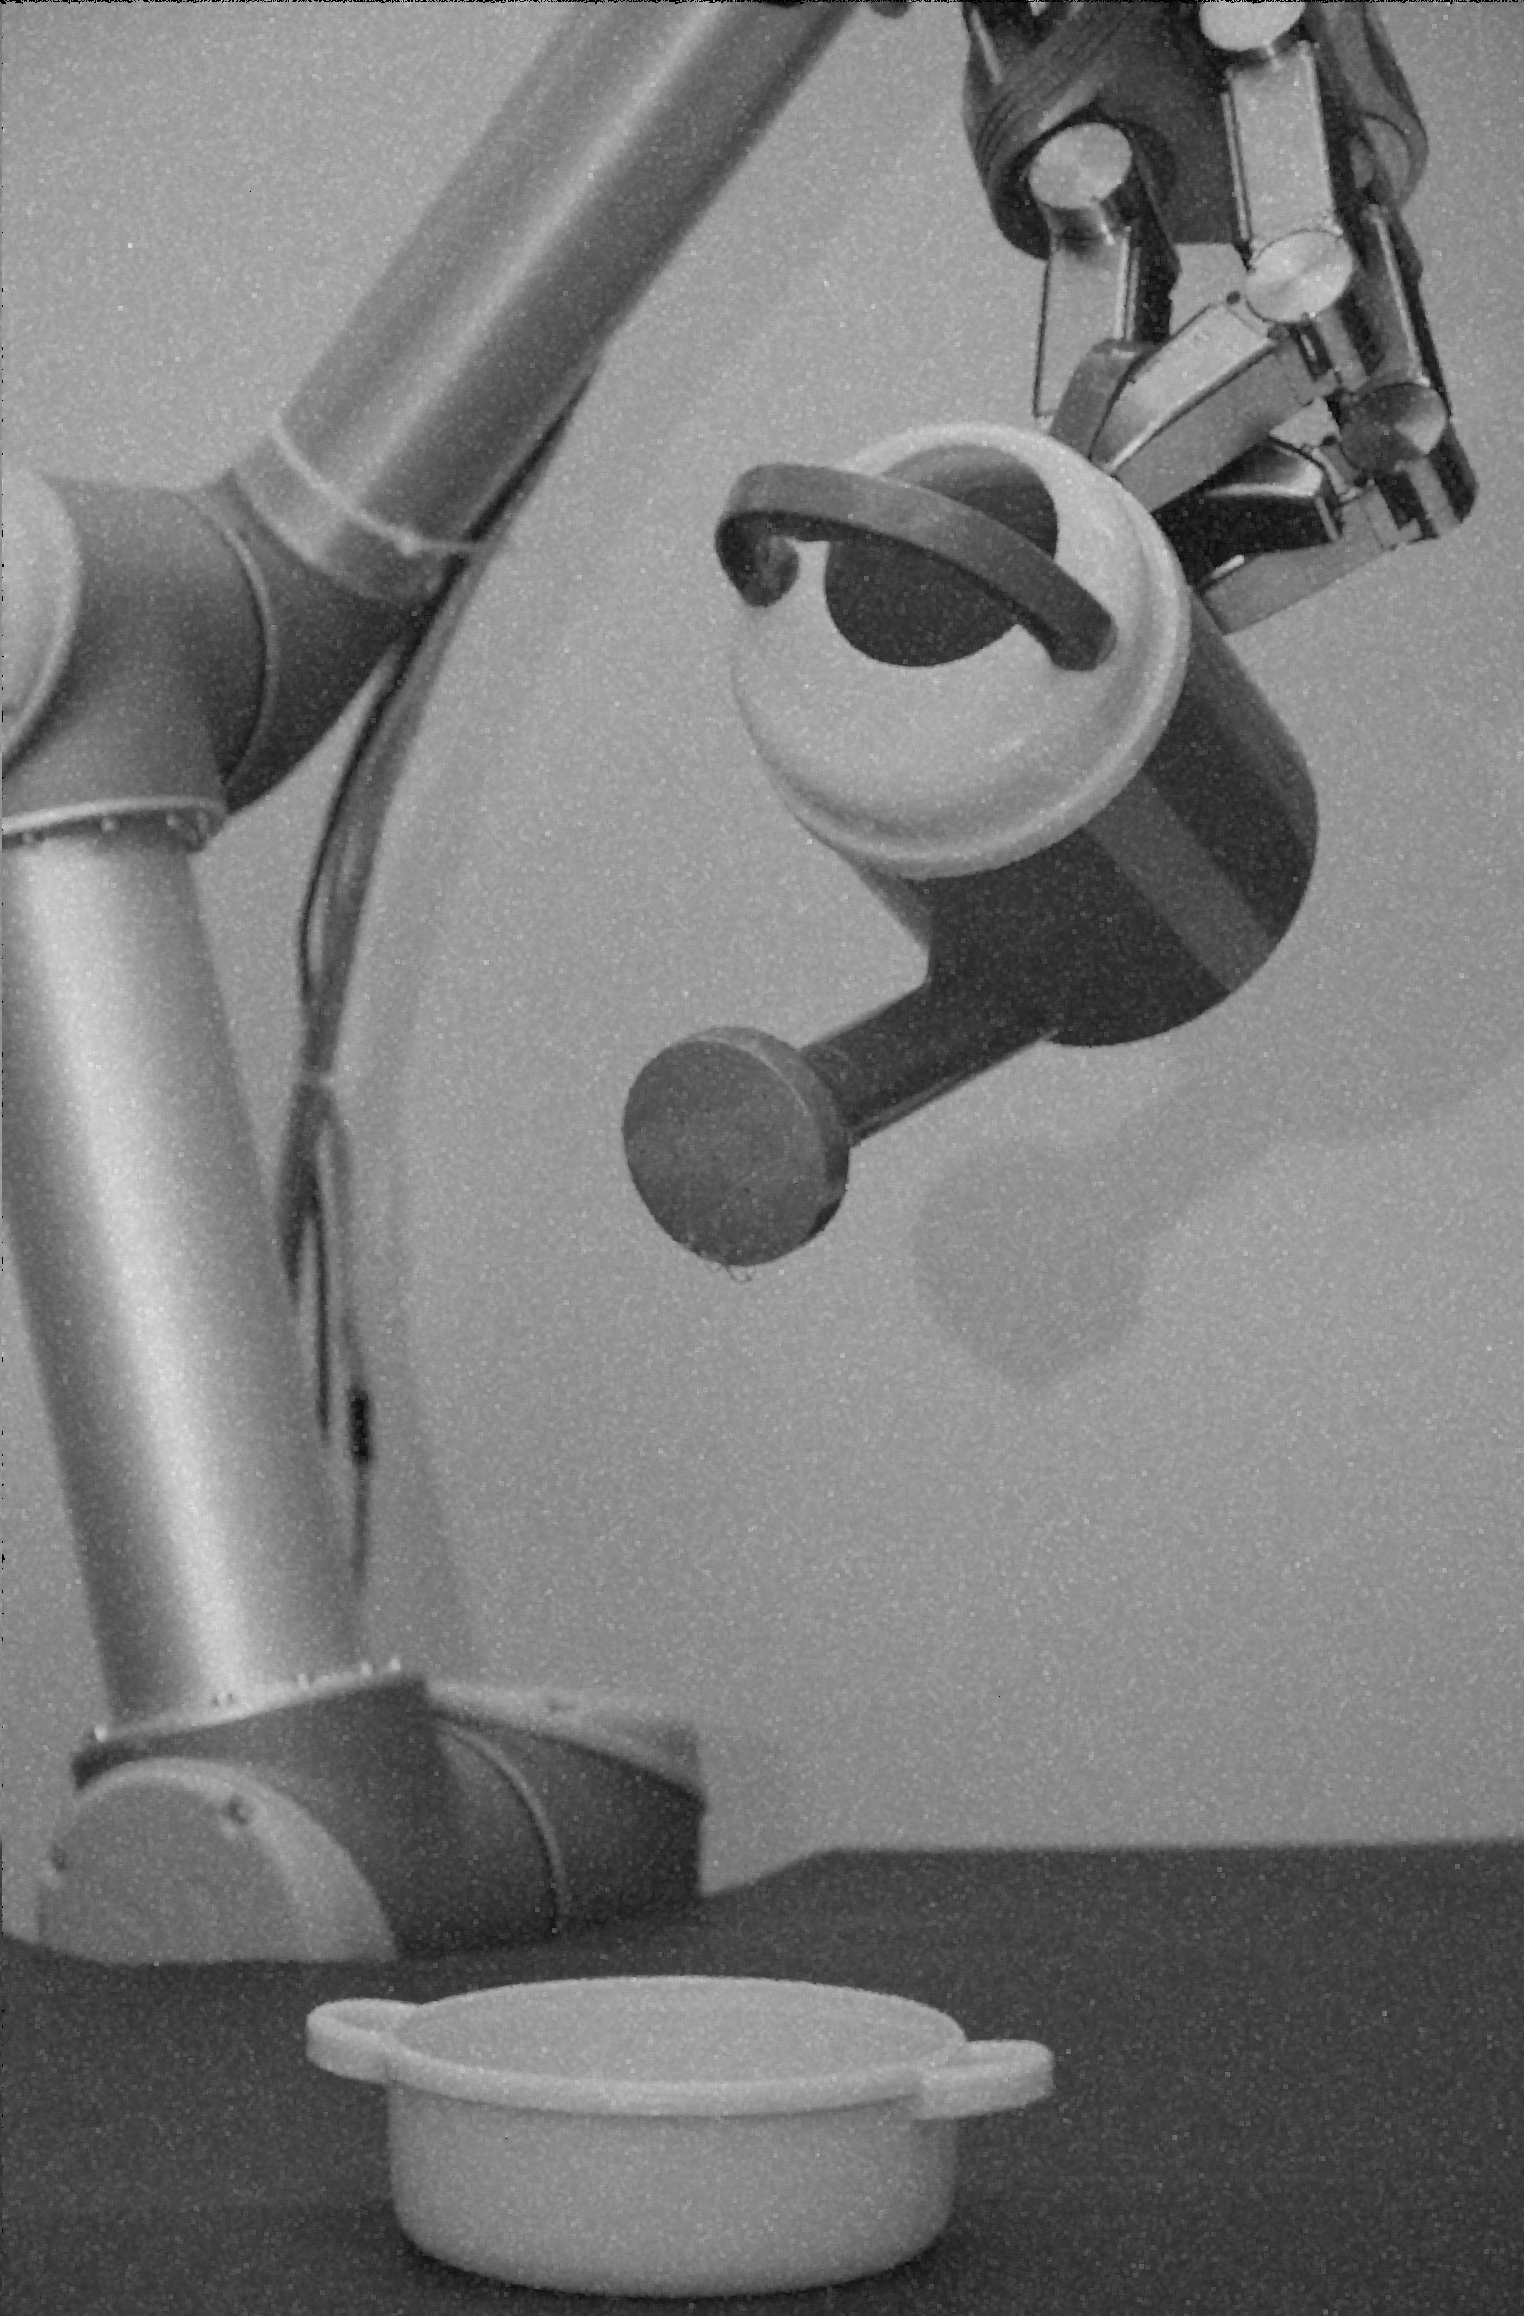
\includegraphics[width=\textwidth]{img1/img_1_gaus_5_1_constrast_strech.png}
        \caption{Contrast stretching applied}
		 %\label{fig:img1_contra11_9}
    \end{subfigure}
     \begin{subfigure}[b]{0.24\textwidth}
        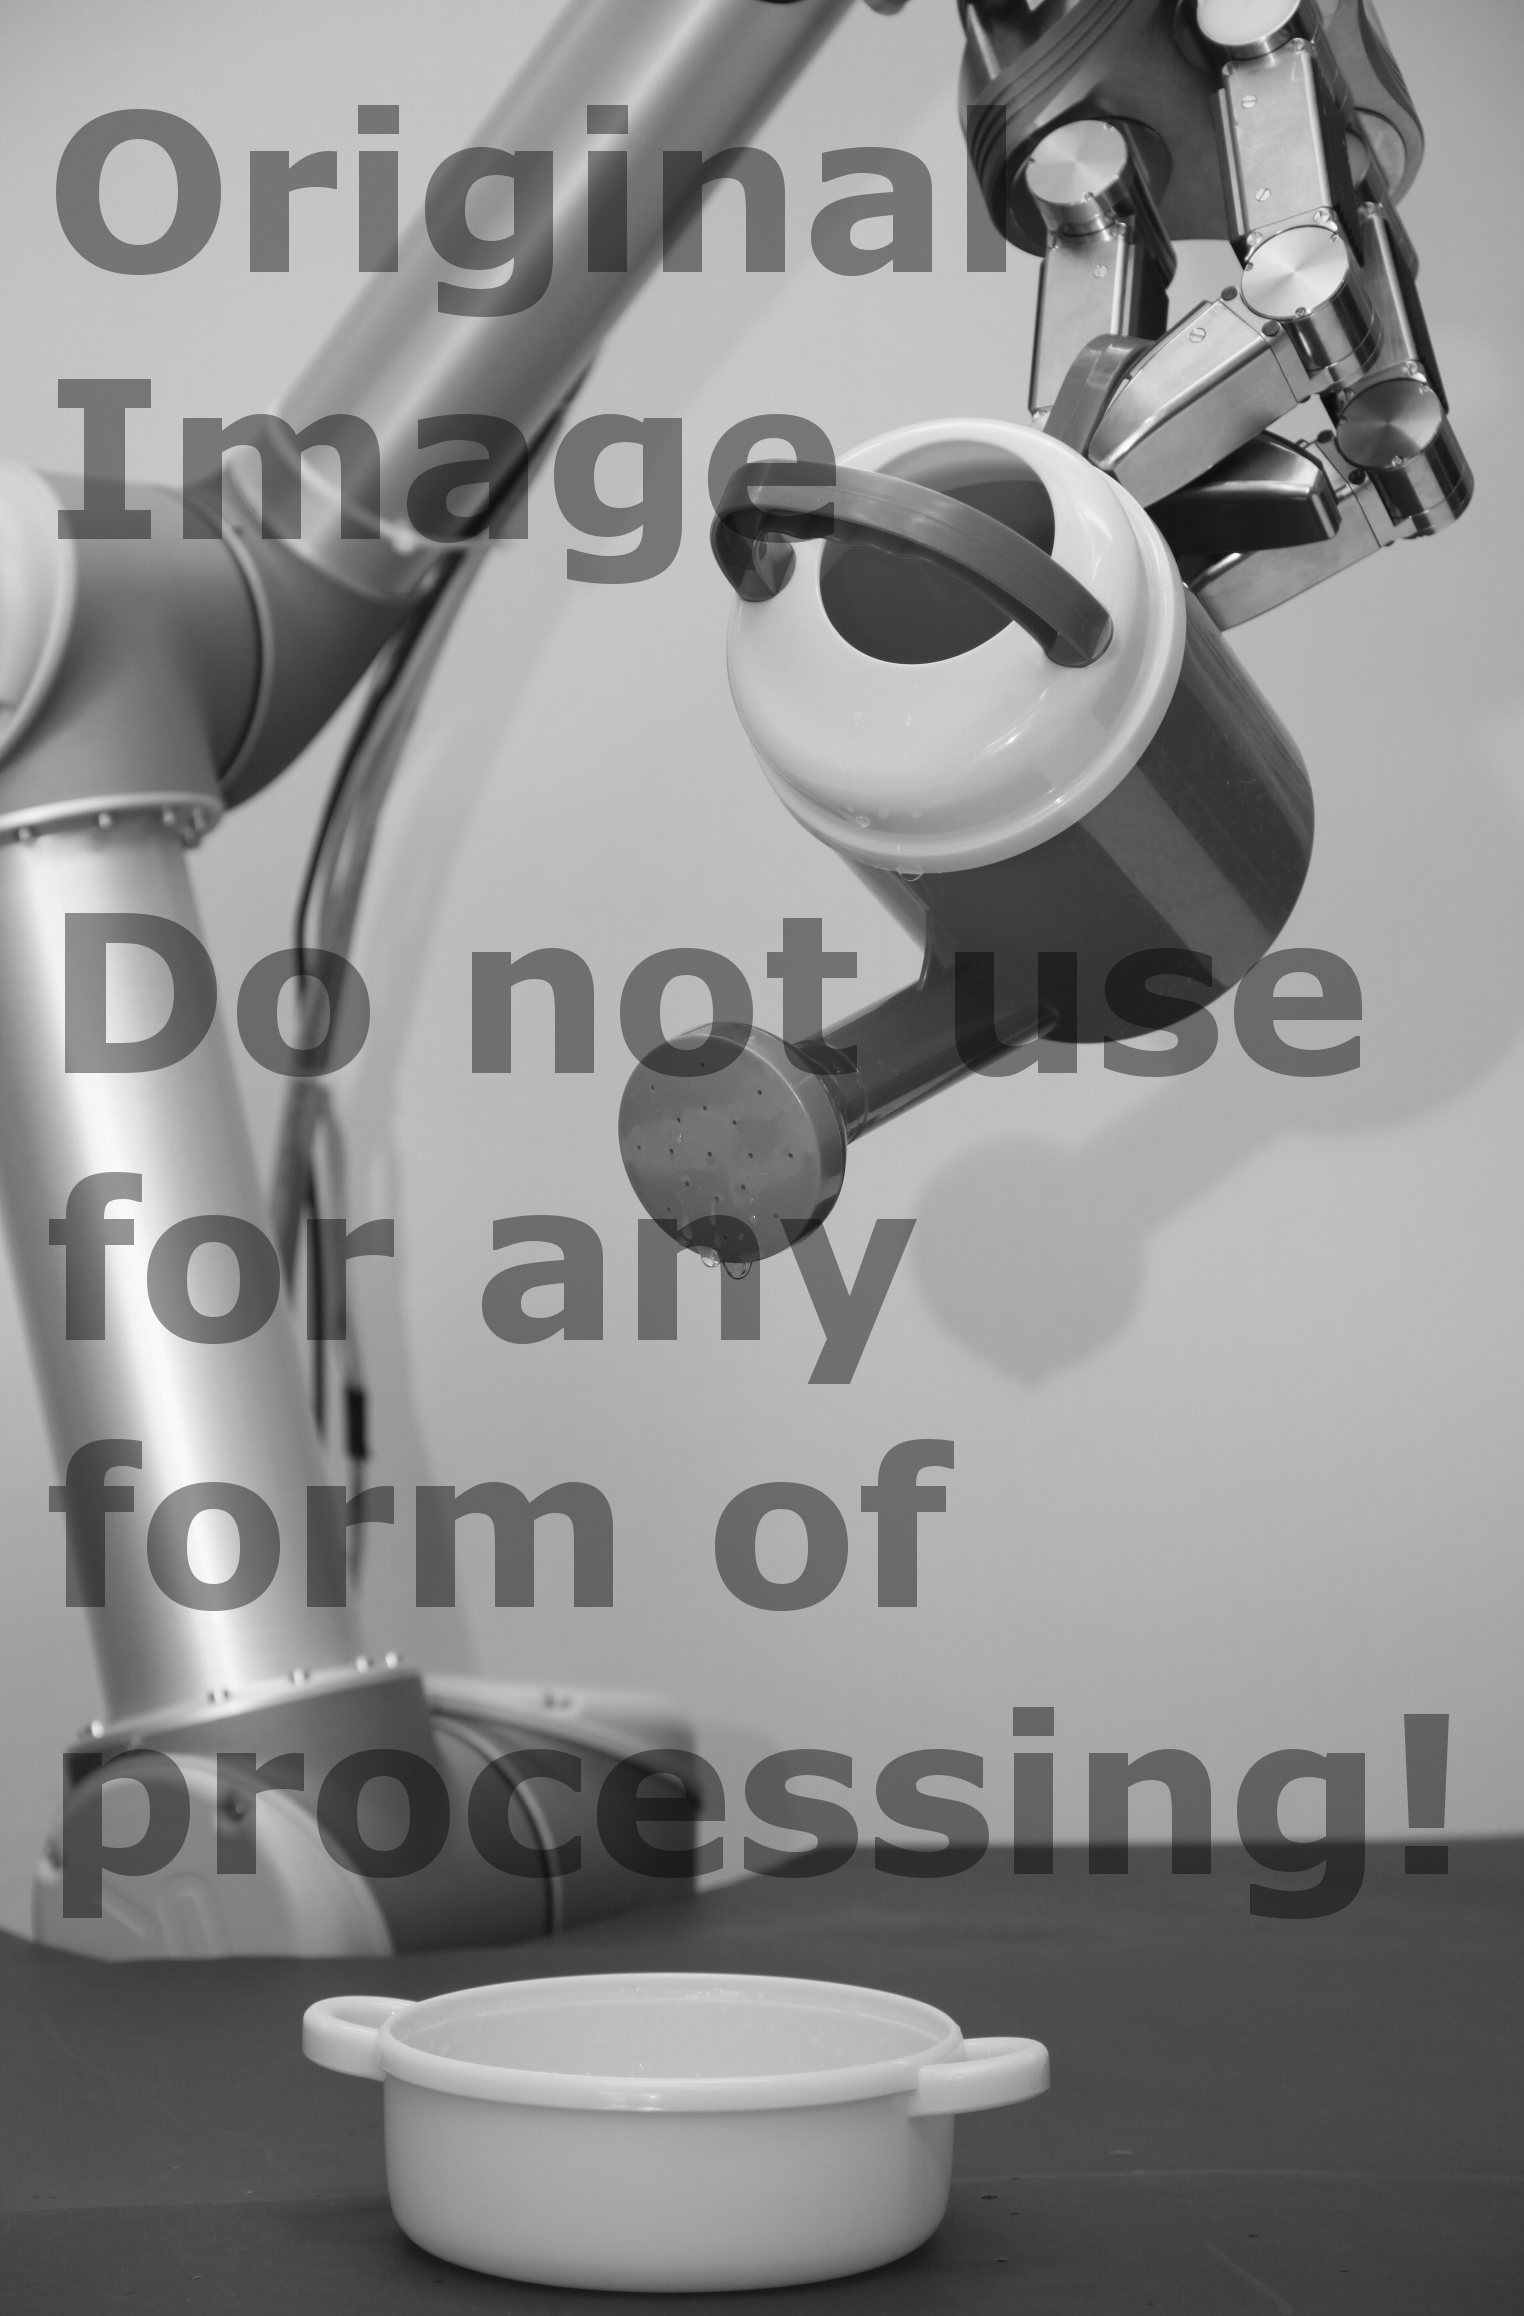
\includegraphics[width=\textwidth]{org.png}
        \caption{Original image}
		 %\label{fig:img1_contra11_9}
    \end{subfigure}   
    \caption{Image restoration process}
    %\label{fig:img1_contra}
\end{figure}


